\chapter {Developing Physics-based Approaches towards PMP Estimation}
\label{ch:JHM}
\externaldocument{appendixJHM}
 
As the time of writing the dissertation, this chapter has been under review for the \textit{Journal of Hydrometeorology}.\\

\bigbreak

\noindent
\hangafter=1
\setlength{\hangindent}{2em}
Chen, X. and Hossain, F., Understanding Model-based Probable Maximum Precipitation Estimation as a Function of Location and Season from Atmospheric Reanalysis. \textit{Journal of Hydrometeorology} (under review).

\vspace{10mm}

\noindent
\textit{\textbf{Abstract}}
 
Extreme precipitation events bring huge societal and economic loss around the world every year, and they have undergone spatially heterogeneous changes in the past half-century. They are fundamental to probable maximum precipitation (PMP) estimation in engineering practice, making it important to understand how extreme storm magnitudes are related to key meteorological conditions. However, there is currently a lack of information that can potentially inform the engineering profession on the controlling factors for PMP estimation. In this study, we present a statistical analysis of the relationship between extreme 3-day precipitation and atmospheric instability, moisture availability and large-scale convergence over the Contiguous US (CONUS). The analysis is conducted using the North America Regional Reanalysis (NARR) and ECMWF ERA-Interim reanalysis data, and a high-resolution regional climate simulation. While extreme 3-day precipitation events across the CONUS are mostly related to vertical velocity and moisture availability, those in the southwestern US mountain regions are also controlled by atmospheric instability. Vertical velocity and relative humidity have domain-wide impacts, while no significant relationship is found between extreme precipitation and air temperature. Such patterns are stable over different seasons and extreme precipitation events of various durations between 1 and 3 days. Our analyses directly help in configuring the numerical models for PMP estimation at a given location for a given storm.

\vspace{20mm}

\section{Introduction}
 
Extreme rainstorms are events that rarely happen and whose magnitudes are far beyond the average climatological statistics. They are responsible for a large fraction of flooding and landslides and bring huge societal and economic losses every year [\textit{Evans et al.}, 2000; \textit{Casagli et al.}, 2006; \textit{Cong et al.}, 2006]. The historical changes in extreme rainstorms are often attributed to global warming [\textit{Min et al.}, 2011], but studies also show that the historical trends of extreme precipitation vary as a function of duration (from hourly to daily) [\textit{Kunkel et al.}, 2013a; \textit{Prein et al.}, 2017]. This difference suggests that the relationship between air temperature and precipitation is not simple. Therefore, a better understanding of the relationship between various atmospheric conditions and precipitation is a necessity.

Extreme rainstorms are also the cornerstone of the engineering design community for water management. Large water management infrastructures have been built to last tens to hundreds of years using Probable Maximum Precipitation (PMP) as a key criterion. PMP is now widely used in the design of these infrastructures all around the world. It is defined as the theoretical greatest depth of precipitation for a given duration that is physically possible over a particular drainage area [\textit{Huschke}, 1959]. During the past several decades, PMP has been mostly estimated through moisture maximization of the extreme rainstorm observations as $PMP={P}\times{PW_m}/{PW_o}$ \textit{[Chreiner and Riedel}, 1978; \textit{World Meteorological Organization (WMO)}, 1986; \textit{Kunkel et al.}, 2013b]. Here $P$ is the observed rainfall amount, $PW_o$ is the observed precipitable water in the same event, and $PW_m$is the observed maximum precipitable water over certain time duration (such as 12 hours).

Although moisture maximization is one of the most widely used techniques for PMP estimation, various studies have investigated the underlying deficiencies in this approach. A consensus that emerges from those studies is that numerical model-based method is expected to be physically superior for estimation of PMP [\textit{Abbs}, 1999; \textit{Tan}, 2010; \textit{Ohara et al.}, 2011; \textit{Stratz and Hossain}, 2014; \textit{Ishida et al.}, 2015; \textit{Chen and Hossain}, 2016]. The numerical approach is based on the physical maximization of a phenomenon relevant to the historical storm reconstruction. A recent study by \textit{Chen and Hossain} [2016] has shown that it is now possible to reconstruct the infrastructure-relevant extreme rainstorms of CONUS after 1948 with acceptable accuracy. However, up to now, there is no consensus on how to physically ``maximize" the historical storms for PMP estimation using numerical model.

The ways to maximize storms as reported in literature can be classified into these categories: 1) disturbance of air moisture through changing air temperature/relative humidity and keeping the atmospheric columns throughout the simulation domain fully moist during the storm events [\textit{Tan}, 2010; \textit{Ohara et al.}, 2011]; 2) disturbance of moisture flux through changing wind speed or wind fields [\textit{Ishida et al.}, 2015]; 3) combination of worst historical environmental conditions [\textit{Tan}, 2010]. One particular issue that makes such techniques appear ad hoc is that there has been no comprehensive study to date that investigates the key atmospheric conditions that affect extreme storms (e.g., moisture availability, atmospheric instability, large-scale convergence). Thus, the engineering community is left without a rational guideline on the use of numerical models for PMP estimation. The information on how extreme historical rainstorms are controlled by environmental conditions is now timely as the engineering community debates and re-evaluates the future risk of water management infrastructures [\textit{Chen and Hossain}, 2016].

There have been various studies on the cause of extreme storms, mostly on selected events. For example, a series of studies on a heavy rainfall event in Mumbai, India, identified the synoptic-scale weather systems and land surface feedback as contributors to this epic event [\textit{Rao et al.}, 2007; \textit{Vaidya and Kulkarni}, 2007; \textit{Kumar et al.}, 2008; \textit{Chang et al.}, 2009]. Similarly, the record-breaking Nashville, Tennessee storm on May 2010 was investigated in \textit{Moore et al.} [2012] and \textit{Durkee et al.} [2012], and it concluded that the storm is a result of interaction between North Atlantic Oscillation, an atmospheric river and strong land surface feedback. These studies now provide a platform for systematic analysis that can be used as a ‘design monograph’ or guide that engineers are so inclined to apply in practice. Some systematic studies have also been done on the general relationship between extreme storms and environmental factors, but most of them only checked the relationship at hourly scale or selected events [\textit{Hand et al.}, 2004; \textit{Hardwick Jones et al.}, 2010; \textit{Mishra et al.}, 2012; \textit{Ducrocq et al.}, 2014].

Other studies approached this problem by systematically checking certain environmental factors [\textit{Davies et al.}, 2013; \textit{Lepore et al.}, 2015]. For example, \textit{Davies et al.} [2013] identified the significant roles of moisture convergence in tropical rainfall events. \textit{Loriaux et al.} [2016] found that atmospheric instability, moisture availability, horizontal wind convergence are all positively related to the hourly peak rainfall intensity in the Netherlands. The rainfall events were treated in a single analysis, and no spatial patterns were analyzed. Some exceptions, such as the study by \textit{Lepore et al.} [2015] that divided the eastern US into four sub-regions, reveal the geographic patterns at a quite coarse scale, and the results are not spatially fine enough to inform the engineering design practice for water management infrastructure. These studies also indicate the usefulness of atmospheric reanalysis products in such analyses. More localized analysis at small sub-regions is required, especially for engineering practice such as PMP estimation.

To address this need, some studies often correlate precipitation with various environmental conditions. Other studies further quantify these correlations as regressions [\textit{Lepore et al.}, 2015]. However, by this approach it is difficult to account for most of the time lags between extreme rainfall intensity and extreme environmental conditions. To avoid the lag issue, our study analyzes the environmental conditions in 72-hour durations, which is also a general standard design period for large water management infrastructures. Also, this correlation/regression approach inexplicitly assumes a fixed relationship between precipitation and environmental factors. For example, \textit{Lepore et al.} [2015] assumed a linear relationship between precipitation and atmospheric instability. This may introduce extra uncertainties in the regression results. To overcome this, in this study we look at a wide range of atmospheric conditions in the frequency space, and make connections between these percentiles by asking the following: when an extreme storm happens, are there any meteorological factors that appear dominant in the same duration?

In this chapter, we examine the extreme precipitation events archived in the North American Regional Reanalysis (NARR) and European Centre for Medium-Range Weather Forecast Interim (ERA-Interim) projects. The use of two reanalysis products helps us to make conclusions that are robust and not subjective to the choice of the product. By extracting the extreme precipitation events across the contiguous US (CONUS) and investigating the atmospheric conditions, we answer the following three PMP-relevant questions:

1.  How has extreme 3-day precipitation changed in the past half-century?

2.  What is the relationship between atmospheric conditions and the extreme rainstorms in the CONUS during 1979-2015 as revealed by reanalysis?

3.  Does the impact of these atmospheric factors show any geographically consistent patterns?

By answering these questions, we find the connections between extreme precipitation and meteorological factors, and use the change in these factors to estimate the change in extreme precipitation. Also, this would reveal how extreme precipitation is likely to behave under the change of these factors, so that simulated ``maximization" is rationalized in numerical models. The paper is organized as follows: In Section 4.2, we introduce the NARR and ERA-Interim data used in this study, as well as the diagnosis variables employed. In Section 4.3, we show the relationship between extreme precipitation amount and various environmental factors during 1979-2015, as well as the geographic distribution of dominant controls on the extreme rainstorms. Further discussions of the results are presented in Section 4.4. Summary and conclusions are presented in Section 4.5.


\section{Data and methods}

\subsection{Reanalysis, simulation, and observation data}

North American Regional Reanalysis (NARR) project is produced by National Centers for Environmental Prediction (NCEP). It reconstructs the weather conditions of North America since 1979 [\textit{Mesinger et al.}, 2006]. This reanalysis is done by assimilating observations from various sources on air temperature, moisture, pressure and wind fields. It also utilizes the surface observations of precipitation, which ensures physically consistent quality in the reconstruction of precipitation. Studies have shown that NARR has an improved representation of the precipitation climatological patterns when compared with previous reanalysis products, especially within the CONUS domain [\textit{Nigam and Ruiz-Barradas}, 2006; \textit{Bukovsky and Karoly}, 2007]. For this reason, NARR has been used in the investigations of the extreme weather events [\textit{Neiman et al.}, 2011; \textit{Wang et al.}, 2016].

ERA-Interim reanalysis is the second generation global reanalysis product from European Centre for Medium-Range Weather Forecasts [\textit{Dee et al.}, 2011]. It is produced using 4-D data assimilation system and benefits from various sources of observation including satellite data. ERA-Interim has been used in various studies on historical extreme weather events including extreme precipitation [\textit{Guan et al.}, 2010; \textit{Pfahl and Wernli}, 2012; \textit{Seneviratne et al.}, 2014]. It has also been used as a historical reference to evaluate the extreme weather in climate models [\textit{Kharin et al.}, 2013].

Some basic information about these two datasets is provided in Table \ref{table:4-1}. In this study, we took the data of 1979-2015 (37 years) and extracted the top fifty 72-hour precipitation events in every grid of the two datasets. At every model grid, we calculated the 72-hour precipitation (MP72 as called thereafter) time series and identified the 50 events with the greatest 72-hour precipitation. To check the quality of reconstructed precipitation climatology, we compared the maximum 72-hour precipitation (i.e., top 1 event) during 1979-2011 against gridded observation [\textit{Livneh et al.}, 2013], as shown in Figure \ref{fig:4-1}. The Livneh gridded daily precipitation data is generated using the gauge observations across the US since 1915, and it is one of the few long-term gridded datasets available. With the higher spatial resolution, NARR captures better the impact of land topography on the atmosphere. This results in higher simulated precipitation from NARR in the west coast and the southeastern US, which is closer to the Livneh data. Figure \ref{fig:4-1}(d) shows the correlation of max 72-hour precipitation between the two reanalysis products with Livneh data. NARR has slightly better performance, though in general the two reanalysis products show the spatial variation reasonably well. In our analysis, we focus on NARR data and take the ERA-Interim as a validation.

\begin{table}[htbp]
	\centering
	\caption{Description of the reanalysis datasets used in Chapter 4}
	\begin{tabular}{cccc}
		\hline
		Dataset & Time range & Spatial resolution & Temporal resolution\\
		\hline
		NARR  & 1979-present  & 32 km / 29 levels  & 3 hourly\\
		\hline
		\multirow{2}{*}{ERA-Interim} & \multirow{2}{*}{1979-present}  & \multirow{2}{*}{0.75 deg / 60 levels}  & 12 hourly ($P$, $CAPE$)\\
		& & & 6 hourly ($PW$, $wind$, $RH$, $T_{air}$)\\
		\hline
	\end{tabular}
	\label{table:4-1}
\end{table}

\begin{figure}[htbp]
	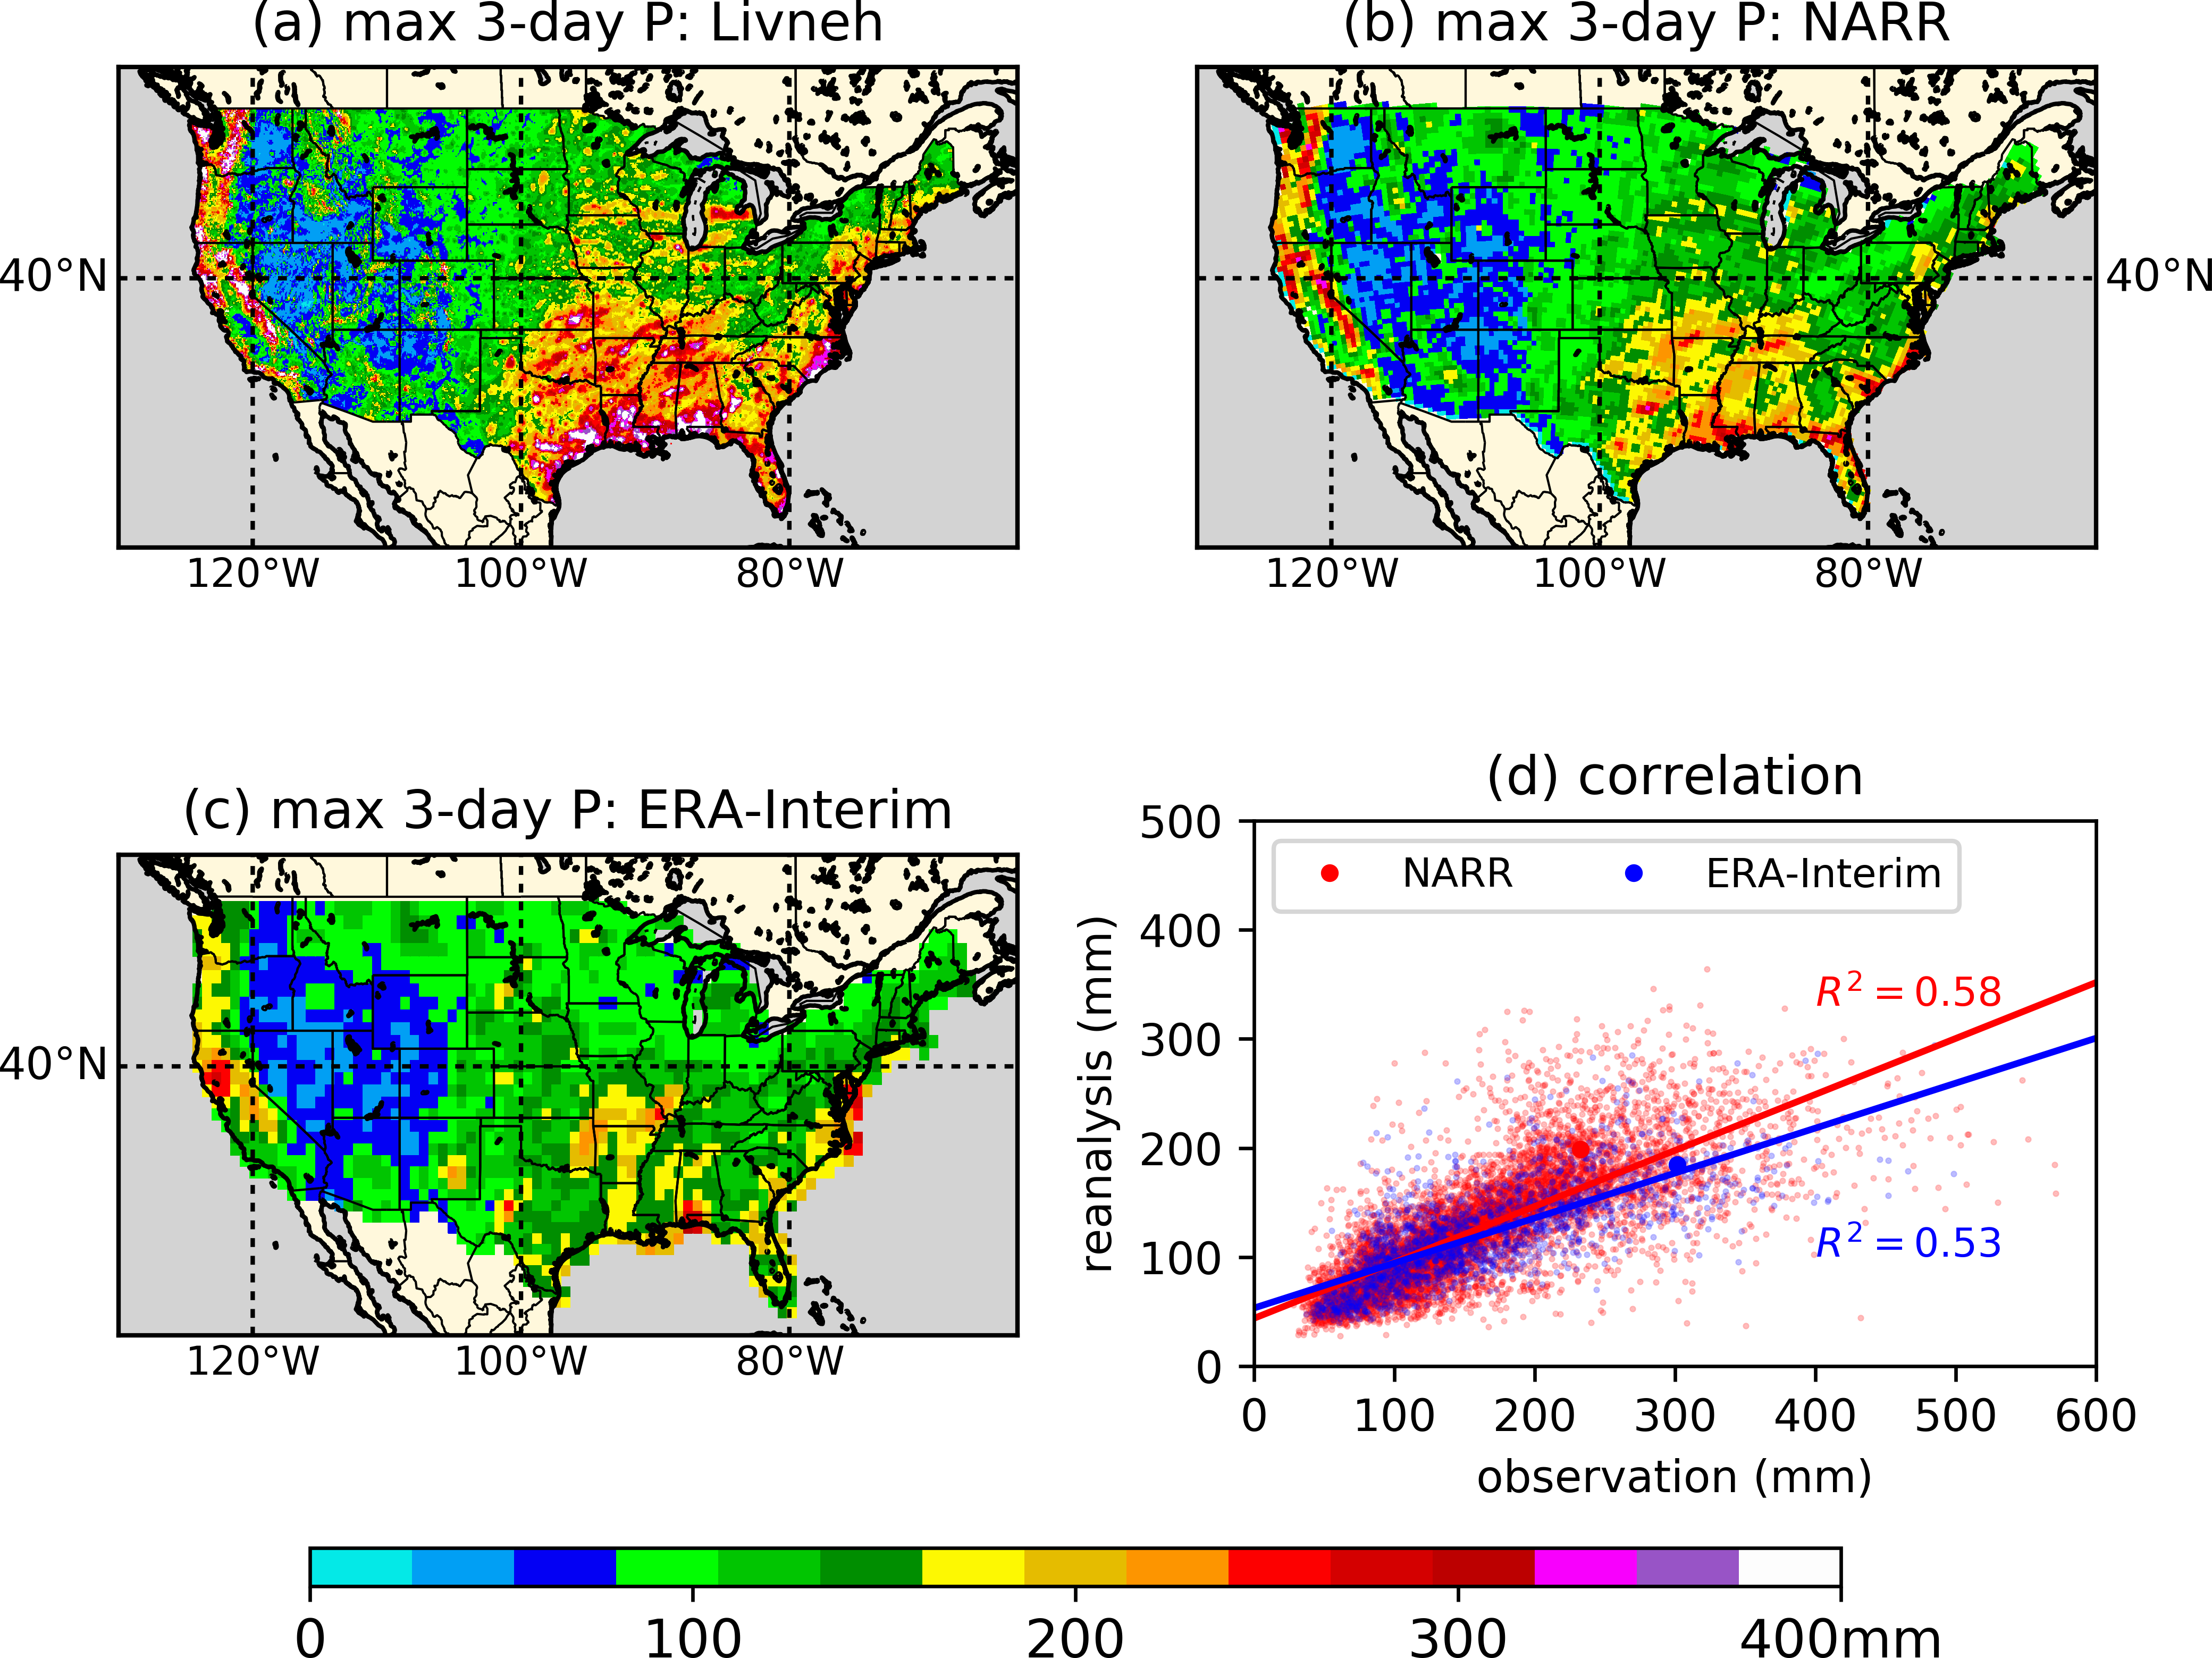
\includegraphics[width=\linewidth]{pics/ch4/fig1.png}
	\caption{Climatologically max 3-day precipitation during 1979-2011 in Livneh gridded observation (a), NARR (b) and ERA-Interim (c). Panel (d) shows the regression between observation and the two reanalysis datasets, where the x-axis is Livneh data, the y-axis is reanalysis data. For this plot, the Livneh data was conservatively regridded to the NARR/Interim model grids.}
	\label{fig:4-1}
\end{figure}

\subsection{Diagnostic atmospheric variables}

Based on previous studies [\textit{Davies et al.}, 2013; \textit{Lepore et al.}, 2015; \textit{Loriaux et al.}, 2016], we first focus on the relationship between extreme precipitation and the following meteorological factors: atmospheric instability, moisture availability, and moisture convergence. These are assumed to be major factors related to extreme precipitation. Therefore, we investigate the roles of the following atmospheric conditions in the initiation and evolution of precipitation: convective available potential energy ($CAPE$), precipitable water ($PW$) and vertical wind velocity ($wind$). $CAPE$ is defined as energy that a parcel of air would have if it were vertically lifted a certain distance in the atmosphere. In this study, we used surface-based $CAPE$, and it is calculated using equation \ref{eq:4-1}, where $Z1$ is the land surface, $Z2$ is the equilibrium level, $T_{v,p}$ is the virtual temperature of the parcel, $T_{v,e}$ is the virtual temperature of the environment, and $g$ is the gravitational constant. $CAPE$ is widely used to indicate the atmospheric instability, and it is useful in predicting severe weather [M\textit{arkowski et al.}, 2002; \textit{Brooks et al.}, 2003]. In general, positive $CAPE$ indicates an unstable condition, and the higher the CAPE value, the more unstable the atmosphere is.

\begin{equation}
CAPE = \int_{Z1}^{Z2} {g\frac{{{T_{v,p}} - {T_{v,e}}}}{{{T_{v,e}}}}dz}
\label{eq:4-1}
\end{equation}

Precipitable water ($PW$) is the vertical integration of moisture in the air column. It is calculated using equation \ref{eq:4-2}, where $x$ is the mixing ratio at the pressure level, $p1$ is the surface pressure, and $p2$ is the uppermost level pressure (100mb in NARR, and 1mb in ERA-Interim). $PW$ indicates the moisture availability for the rainstorm, and in heavy rainstorm events, moisture that is several times of PW can be depleted.

\begin{equation}
PW = \frac{1}{{\rho g}}\int_{p1}^{p2} {xdp}
\label{eq:4-2}
\end{equation}

Vertical wind ($wind$) is directly taken from reanalysis fields, presented as the velocity between pressure levels. From the mass balance perspective, the strength of vertical velocity is also an approximation of the large-scale horizontal convergence (LSC). Our analysis suggests that the greatest vertical velocity happens at 700mb in the MP72 duration. This is in agreement with earlier studies of mid-latitude storms [\textit{Loriaux et al.}, 2016], and in the following analysis, we will analyze the vertical velocity at 700mb, as it is most related to the precipitation process.

$CAPE$, $PW$, and $wind$ represent a summary of atmospheric conditions. To check the role of driving variables in the MP72 process, we also consider relative humidity ($RH$) and air temperature. Specifically, temperature averaged between 850mb and 500mb ($Tavg$) is used to present ``general air temperature", and the temperature difference between 850mb and 500mb ($Tdiff$, $T_{850mb}-T_{500mb}$) is used to present vertical temperature gradient.

\subsection{Analysis approach}

For analysis of long duration events (i.e. multiple days), one difficulty is to define a state for atmospheric conditions that are representative for the storm duration. Therefore, we use frequency analysis to check the extent to which the atmospheric variables are extreme. Figure \ref{fig:4-2} depicts the procedures, and we give a step by step description here. First, at each grid (e.g., the blue grid in figure \ref{fig:4-2}a), we compute the 3-day cumulative precipitation time series from reanalysis data (NARR or ERA-Interim) and collect the top 50 most severe 3-day precipitation events at every model grid during 1979-2015 (figure \ref{fig:4-2}b). At this grid, we also compute the Cumulative Distribution Function (CDF) of factor $X$ ($CAPE$, $PW$, $wind$, $RH$, $Tavg$, or $Tdiff$) using 1979-2015 records, as the blue lines in Figure \ref{fig:4-2}c-e. Then for each of these 50 events, we overlay the values of X in the MP72 duration on the CDF curves. From these combined plots we then infer whether this variable also reaches extreme condition. For the example storm in figure \ref{fig:4-2}, the analysis indicates that PW and wind stay persistently high and they are controlling the magnitude of this storm. Compared with the studies where only the peak rainfall hour (or the surrounding 12 hours) environmental conditions are checked [\textit{Mishra et al.}, 2012; L\textit{oriaux et al.}, 2016], we do not focus on a specific hour, but rather the entire 72-hour duration. This is expected to reduce the bias in the results that are caused by the time lag between peak rainfall and extreme environmental conditions.

\begin{figure}[htbp]
	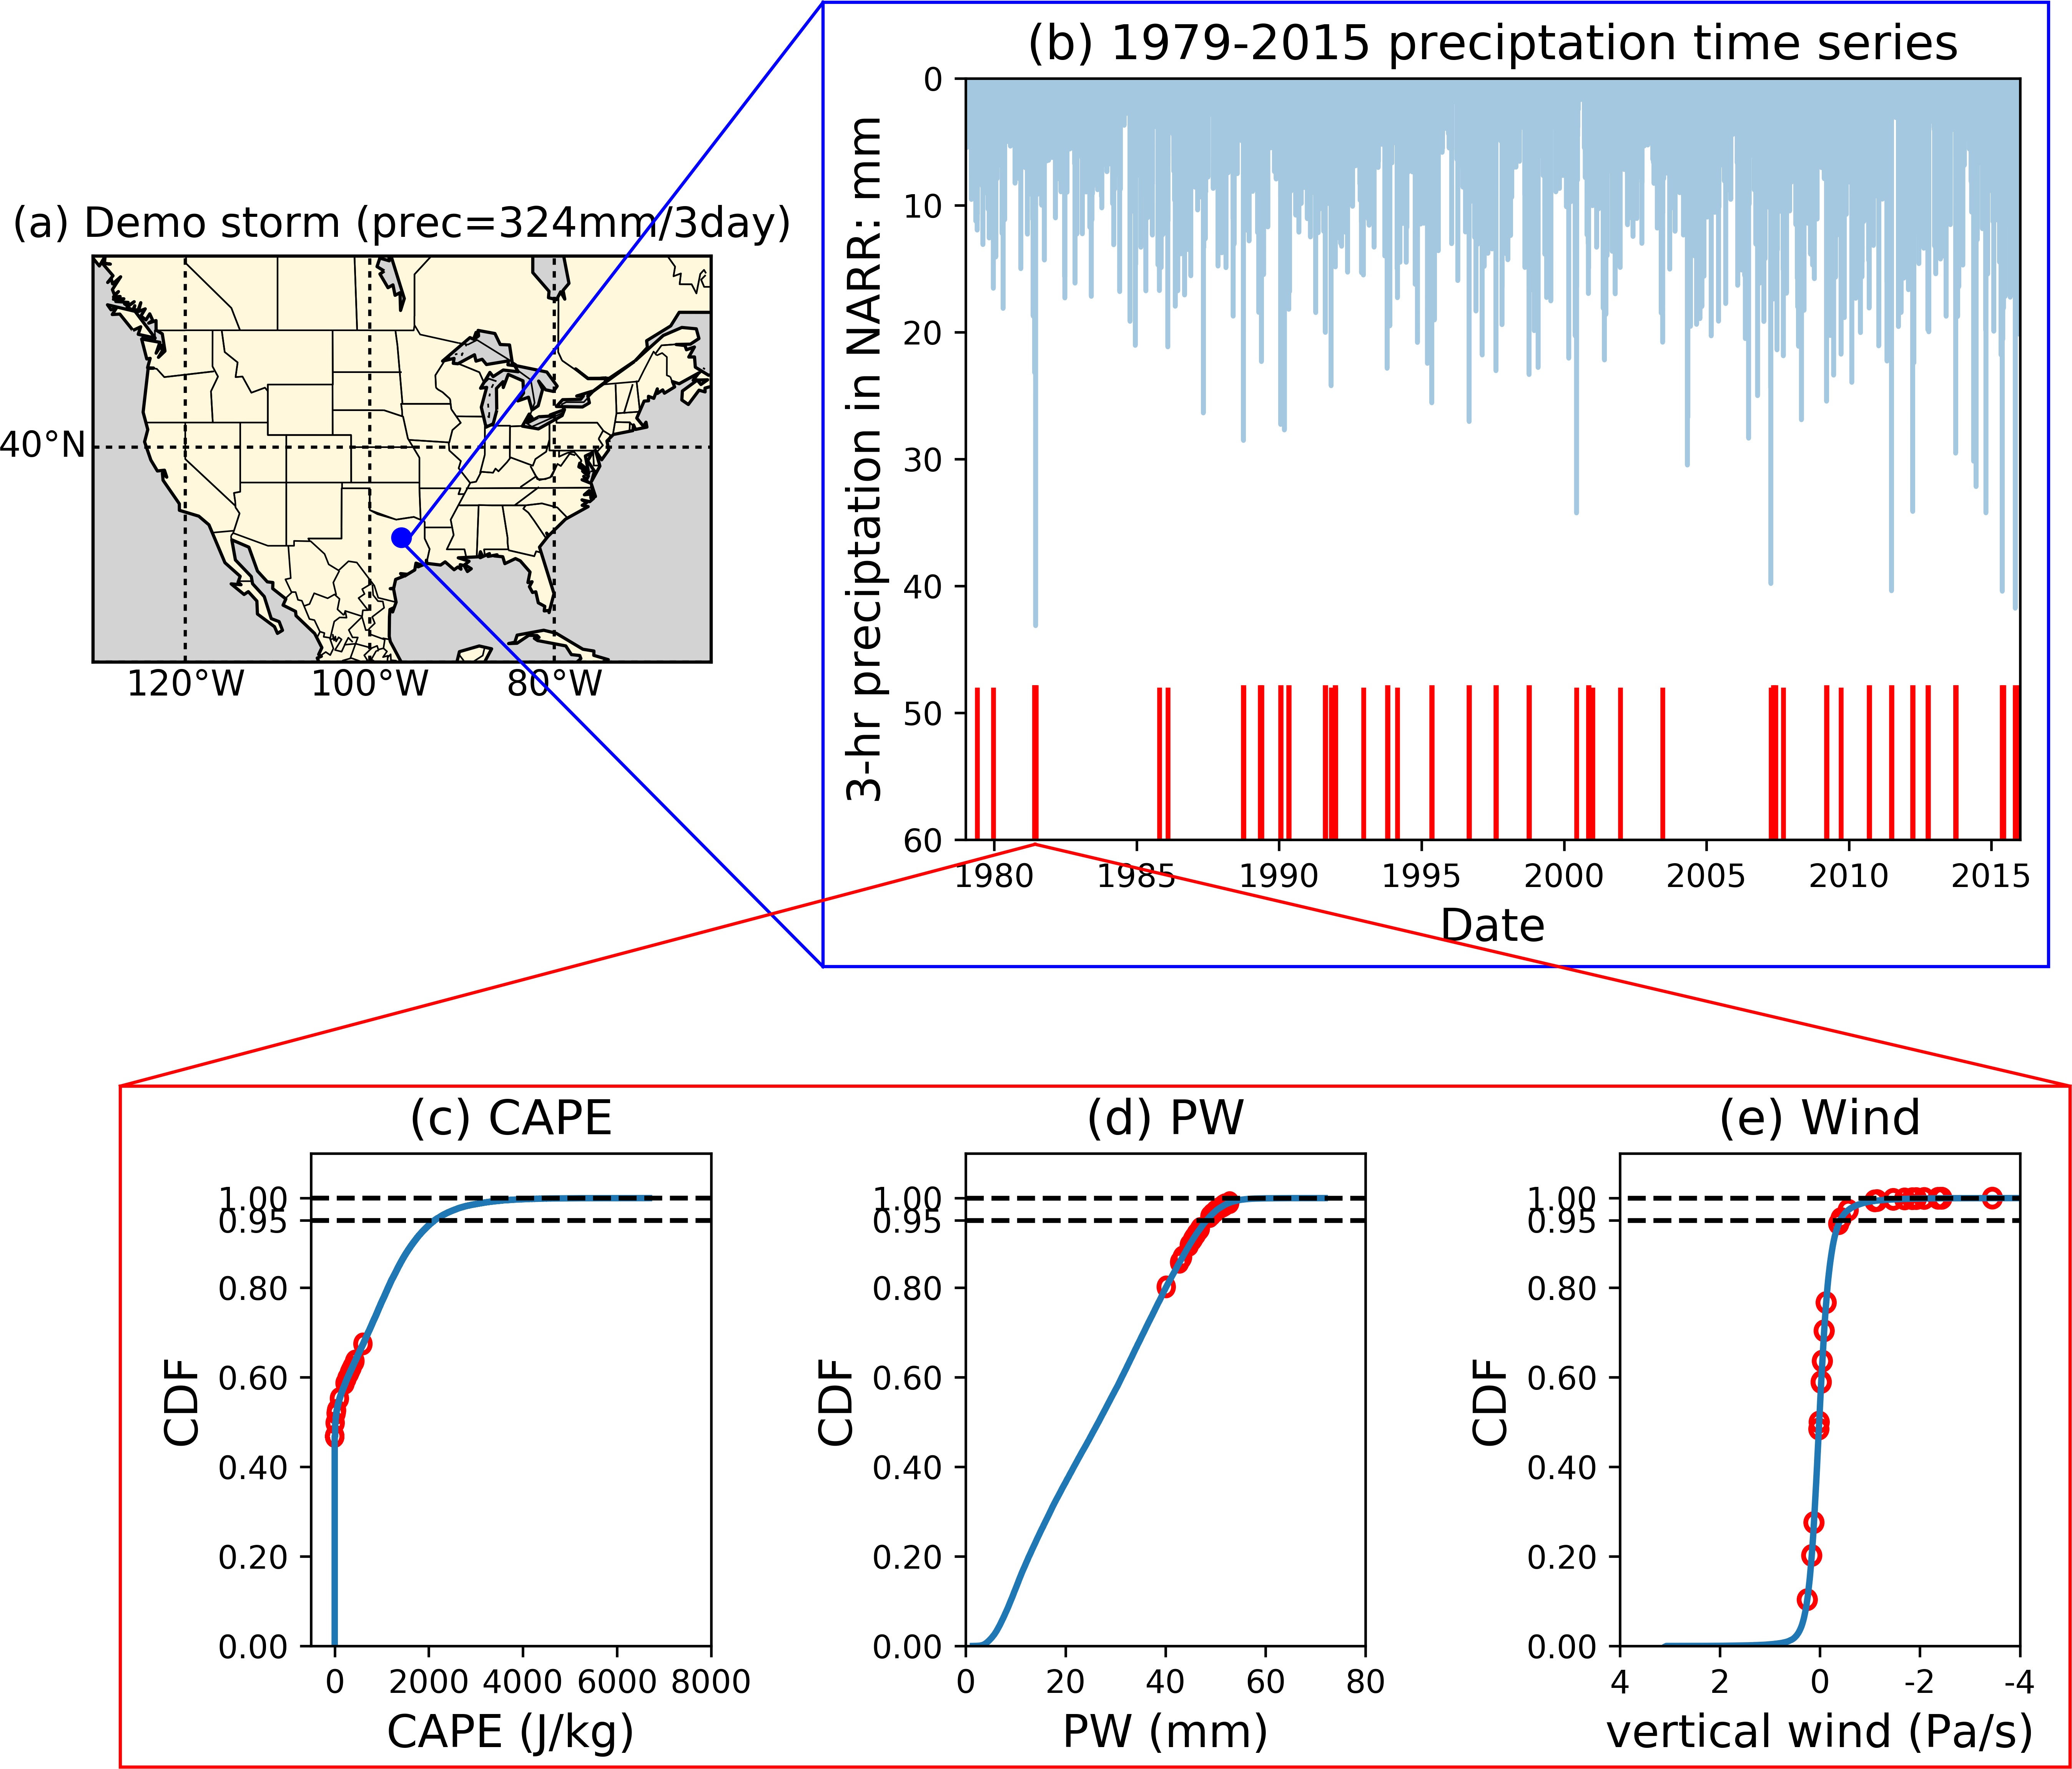
\includegraphics[width=\linewidth]{pics/ch4/fig2.png}
	\caption{Demonstration of frequency-based analysis. From a given grid, such as the blue point in panel (a), we can obtain the precipitation time series from the reanalysis (NARR or ERA-Interim) as shown in panel (b). Then we can identify the top 50 72-hr events with greatest rainfall amount, These 50 periods are shown as red bars in panel (b). From 36-year reanalysis data, we can also obtain the climatology (Cumulative Distribution Function) of $CAPE$, $PW$, and $wind$ as the blue curves in panel (c)-(e). Red dots reflect the conditions of these factors in one 72-hour storm duration. If we define CDF=95\% (dash lines) as the threshold of the extreme condition, it shows that in the 72-hour duration, $PW$ and vertical $wind$ are persistently high, and we call them the controlling factors of this event. At one grid, if a factor controls most of the top 50 events, then it is defined as the dominant control of the extreme storms at this grid.}
	\label{fig:4-2}
\end{figure}

To quantify these environmental controls, we take the $CDF\geq95\%$ (we will call this as parameter p1 thereafter) as the threshold of extreme condition (the dash lines in figure \ref{fig:4-2}c-e). If factor $X$ stays extreme (i.e., $CDF\geq95\%$) for over 15\% (parameter p2) of the MP72 duration (i.e., $\geq4$ snapshots for 3-hr data, or $\geq2$ snapshots for 6-hr data), we define this event as controlled by $X$. Our choice of p1=95\% and p2=15\% may appear somewhat arbitrary. However, our sensitivity tests (figure \ref{fig:4-S1}) indicate that the difference in the results is marginal when the analysis is performed with p1 between [90\%, 99\%] and p2 between [10\%, 20\%]. Besides, our goal here is not to quantify the specific physical trigger but rather to identify the one that is statistically most prevalent (or dominant) at given geographic location. By comparing the percentage of the top 50 events that are controlled by each factor, we can define the dominant physical control as the one controlling most events. The above analyses are based on the full records during 1979-2015, and the year-around dominant controls can be derived. By applying the analysis at seasonal scale, i.e., using only the records and climatology information in the given season, we also investigate the seasonal variability of these physical controls.

Following the same analysis framework but on precipitation of different durations (e.g., 1 day, or 2 days), we can also investigate the dominant control of these different precipitation events.

\subsection{Estimation of precipitation change based on dominant meteorological factor}

The above analysis reveals how extreme precipitation at a given location is related to the meteorological conditions. If factor $X$ plays a dominant role, then it is reasonable to expect that extreme precipitation will exhibit similar trend as factor $X$. Due to the different magnitude and unit of measurement for different factors, this approach can only give binary info (i.e., increase or decrease) in the precipitation trend.


\section{Results}

\subsection{Historical changes in extreme 3-day precipitation}

\begin{figure}[htbp]
	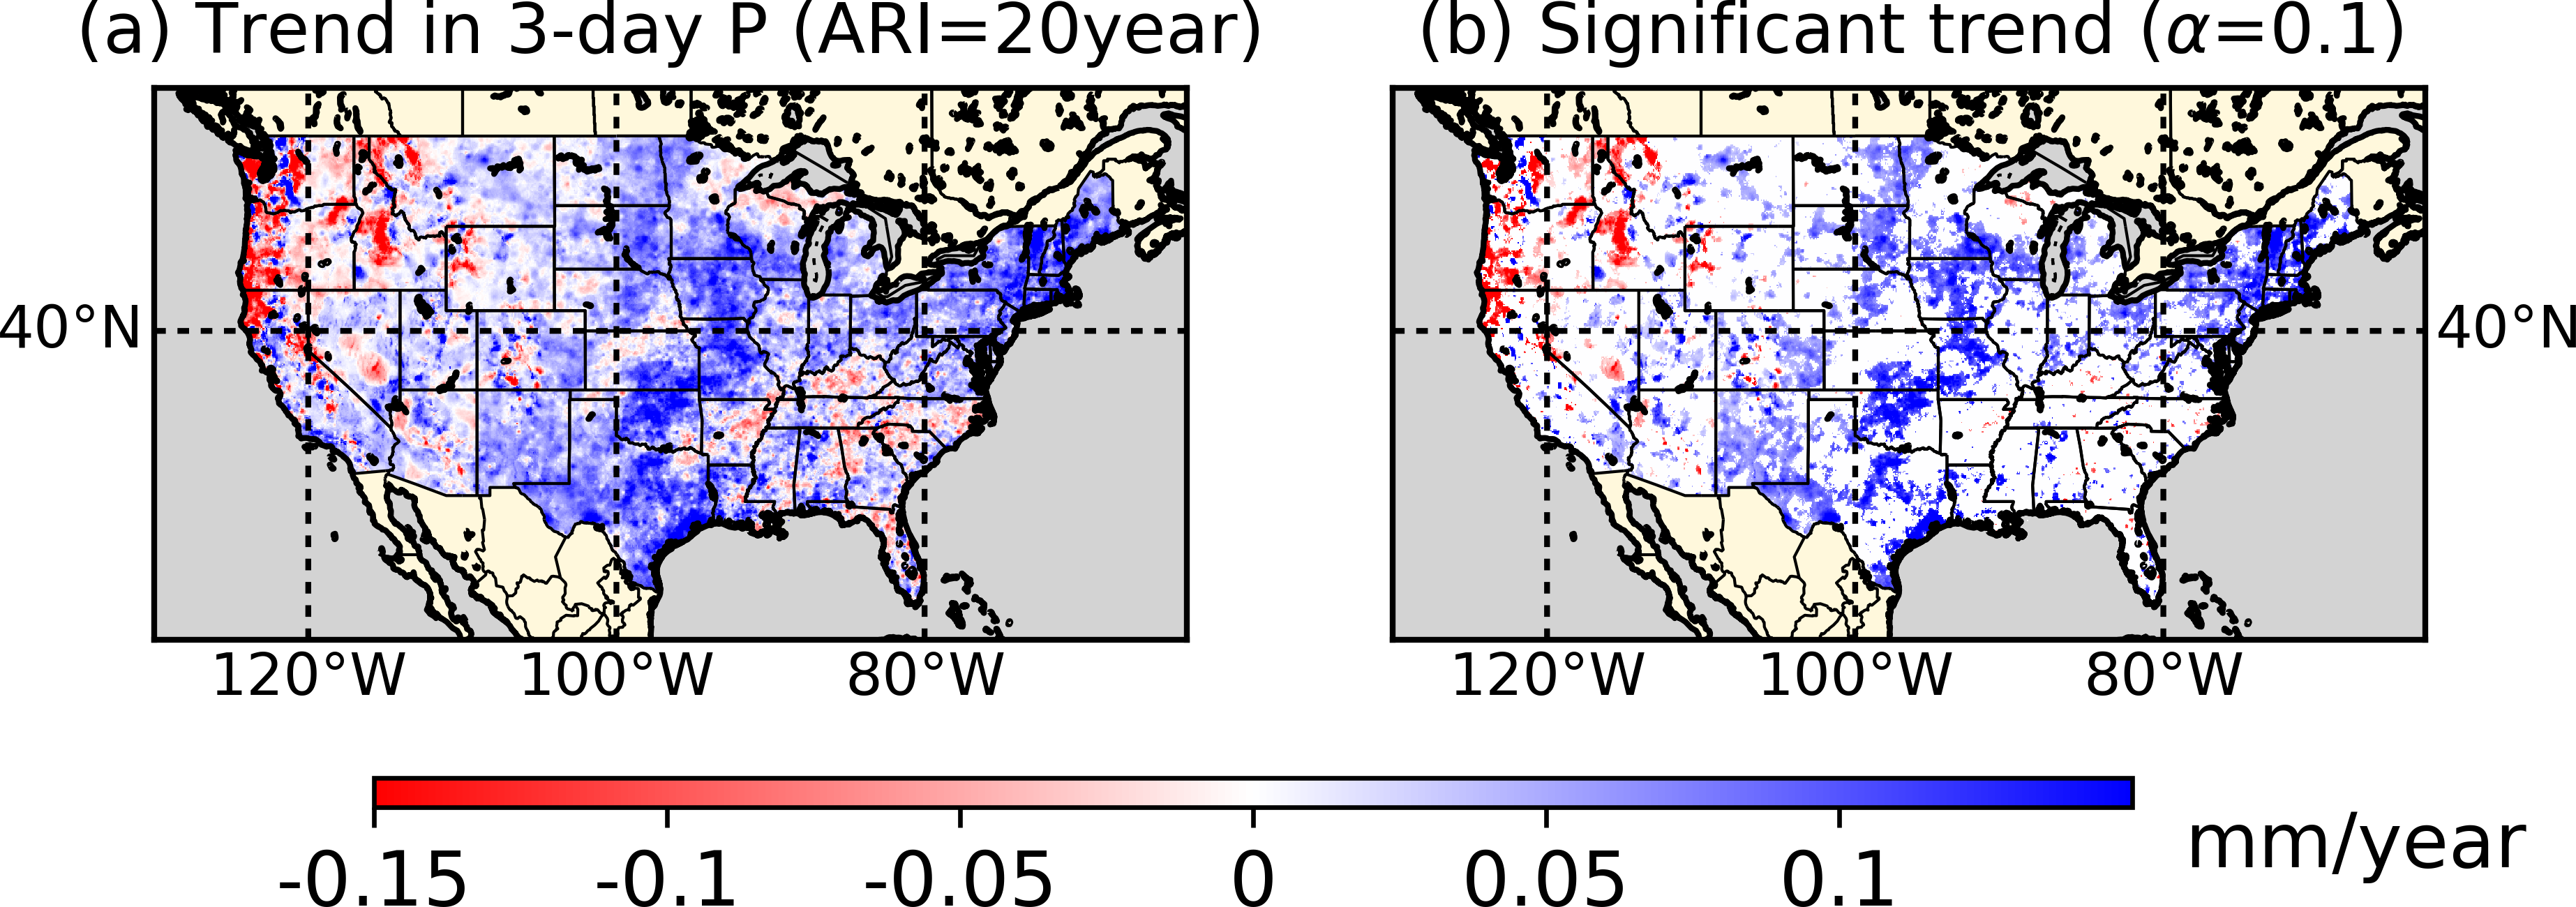
\includegraphics[width=\linewidth]{pics/ch4/fig3.png}
	\caption{Historical trends in extreme 3-day precipitation (taken as 20-year Average Return Interval, ARI) between 1948-2010. The trend is calculated using annual 20-year ARI 3-day precipitation series between 1948-2010 observation. (a) shows the trends from linear regression, and (b) only keeps the grids where the Mann-Kendall test shows a significant trend (at $\alpha=0.1$ level).}
	\label{fig:4-3}
\end{figure}

Figure \ref{fig:4-3} shows the trend of extreme 3-day precipitation between 1948-2010, from gridded observation data [\textit{Livneh et al.}, 2013]. This 1/16 degree dataset is available from 1915, but due to limited raw gauge data availability before 1948, we only analyzed the data after 1948. To check the trend during 1948-2010, for each year the 20-year average return interval (ARI) value was computed using the 3-day precipitation data in this year. Then linear regression was applied to estimate the trend (panel \ref{fig:4-3}a), and Mann-Kendall test was applied to check the significance of these trends (panel \ref{fig:4-3}b). Panel \ref{fig:4-3}b only renders the grids where the trends are statistically significant under Mann-Kendall test ($\alpha=0.1$). It shows high spatial variation in the extreme precipitation trends, with mainly the central US showing more significant increasing trends. Extreme precipitation in the northwestern US and the southeastern US shows decreasing trends, but the trends in the southeastern US are not significant.

Compared with changes in hourly and daily extreme precipitation found in previous studies [\textit{Kunkel et al.}, 2013a; \textit{Prein et al.}, 2017], figure \ref{fig:4-3} shows higher spatial heterogeneity. This suggests that the sensitivity of long-duration (i.e., longer than one day) extreme events to the past global warming is not the same across the CONUS, and some of them may be sensitive to other climate variables.

To connect the changes in extreme precipitation to meteorological conditions, we also computed the 1979-2015 trends of the NARR meteorological factors ($CAPE$, $PW$, $wind$, $RH$, $Tavg$, and $Tdiff$) using the same method (figure \ref{fig:4-S2}). A visual comparison suggests the precipitation change (figure \ref{fig:4-3}a) pattern mostly resembles the vertical wind change (figure \ref{fig:4-S2}c). Previous studies indicate that although changes in extreme precipitation follow the Clausius-Clapeyron relation, it can be different when local moisture convergence (strong wind) takes place [\textit{Trenberth}, 1999; \textit{Trenberth et al.}, 2003]. Thus it is necessary to look into the relationship between extreme precipitation and individual factors.

\subsection{How is 3-day extreme precipitation related to atmospheric conditions?}

\begin{figure}[htbp]
	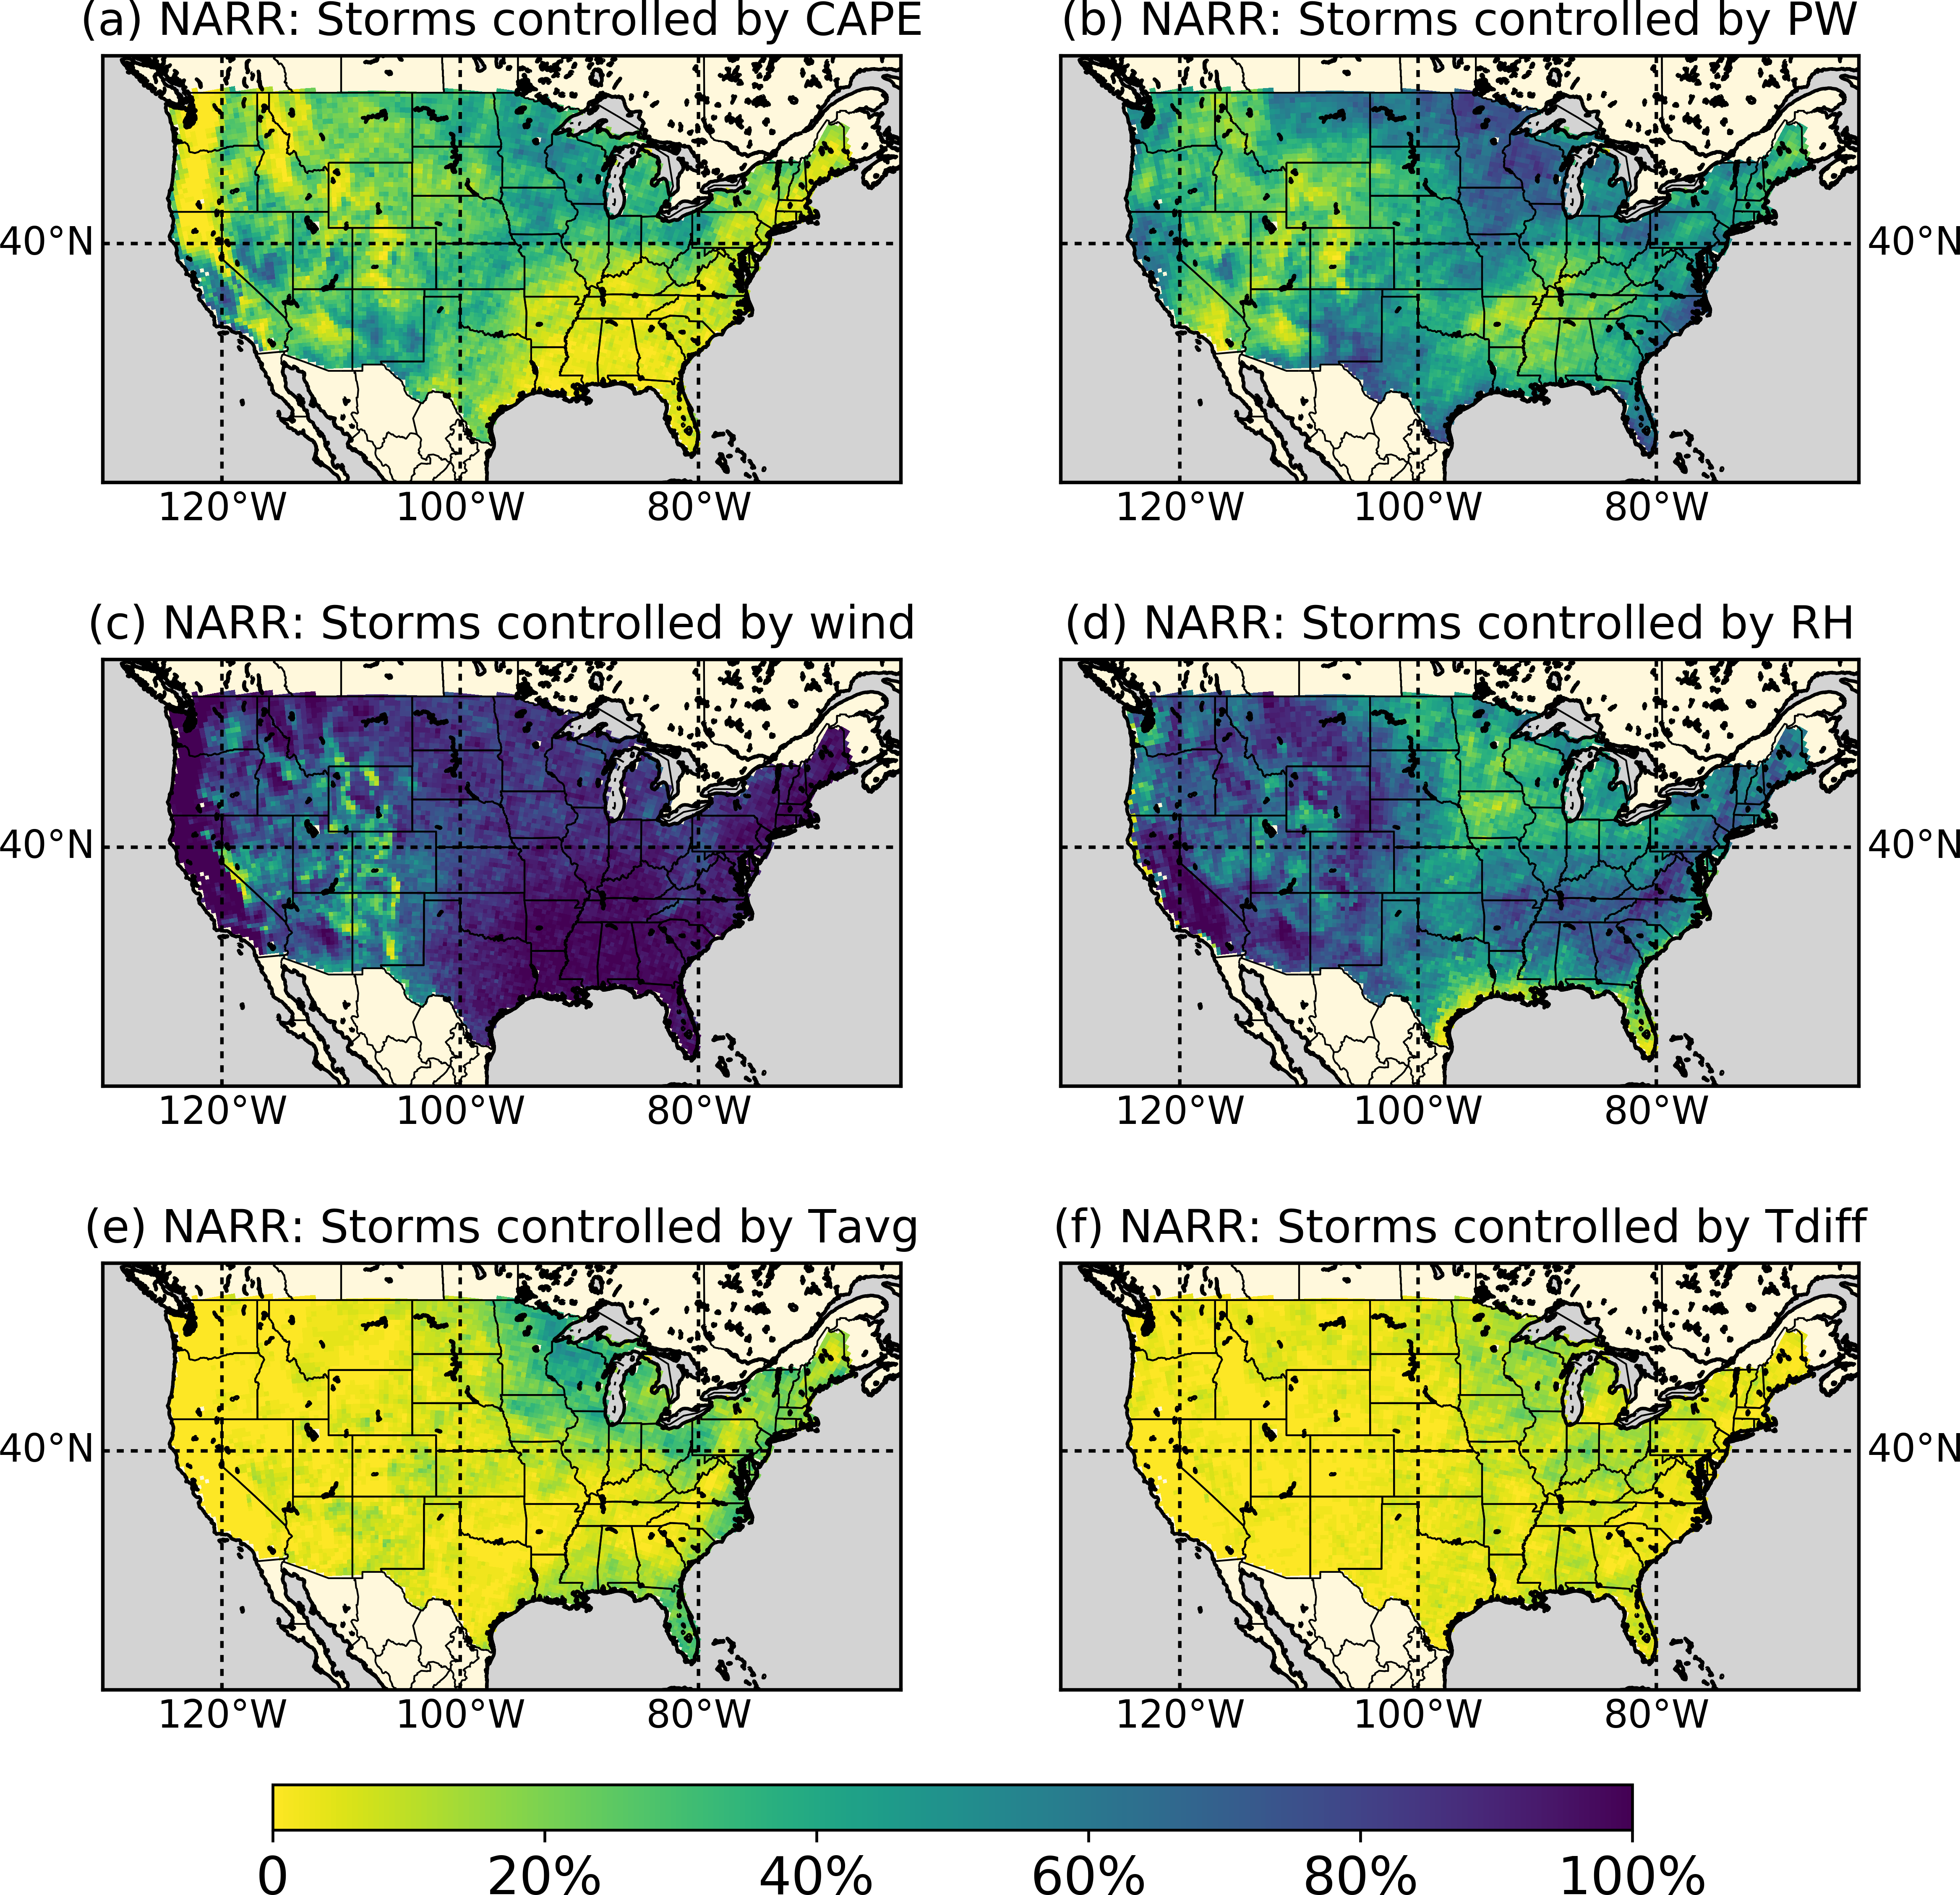
\includegraphics[width=\linewidth]{pics/ch4/fig4.png}
	\caption{Percentage of top 50 extreme precipitation events that are related to extreme $CAPE$ (a), $PW$ (b), $wind$ (c), $RH$ (d), $Tavg$ (e), and $Tdiff$ (f) during 1979-2015, from NARR. This reflects how many of top 50 extreme 3-day rainfall events at a given grid are controlled by this meteorological factor.}
	\label{fig:4-4}
\end{figure}

Figure \ref{fig:4-4} shows the percentage of top 50 local extreme precipitation events that are related to extreme $CAPE$, $PW$, and vertical $wind$ from NARR data. Overall vertical wind velocity has the greatest impact on the extreme precipitation, and this is reasonable given that vertical motion triggers moisture condensation. It is necessary to note the presence of strong vertical velocity in the west coast and the southeastern US is different, which features atmospheric river systems and mesoscale convective systems (cyclones), respectively. Regarding this ``absolute impact", both $CAPE$ and $PW$ have similar patterns: they are closely related to extreme precipitation in the central US, but less so in the west coast and the southeastern US. The southeast region experiences high CAPE around the year (figure \ref{fig:4-S3}a), so it is not a particularly important factor in the extreme precipitation occurrences. In the northwest region, most of the extreme precipitation events are in wintertime, when the air is cold and stable. Also, they are mainly atmospheric river landfall events where abundant moisture is raised and condenses along the coastal Cascade Range. Thus $CAPE$ does not play a key role there. The fact that extreme precipitation is more related to vertical wind velocity than $PW$ is because vertical wind also implies large-scale horizontal convergence, which brings in moisture from the surrounding area in the precipitation process. This is in agreement with findings from previous studies that during the extreme rainfall events, the consumed moisture is several times of PW [\textit{Kunkel et al.}, 2013b].

\begin{figure}[htbp]
	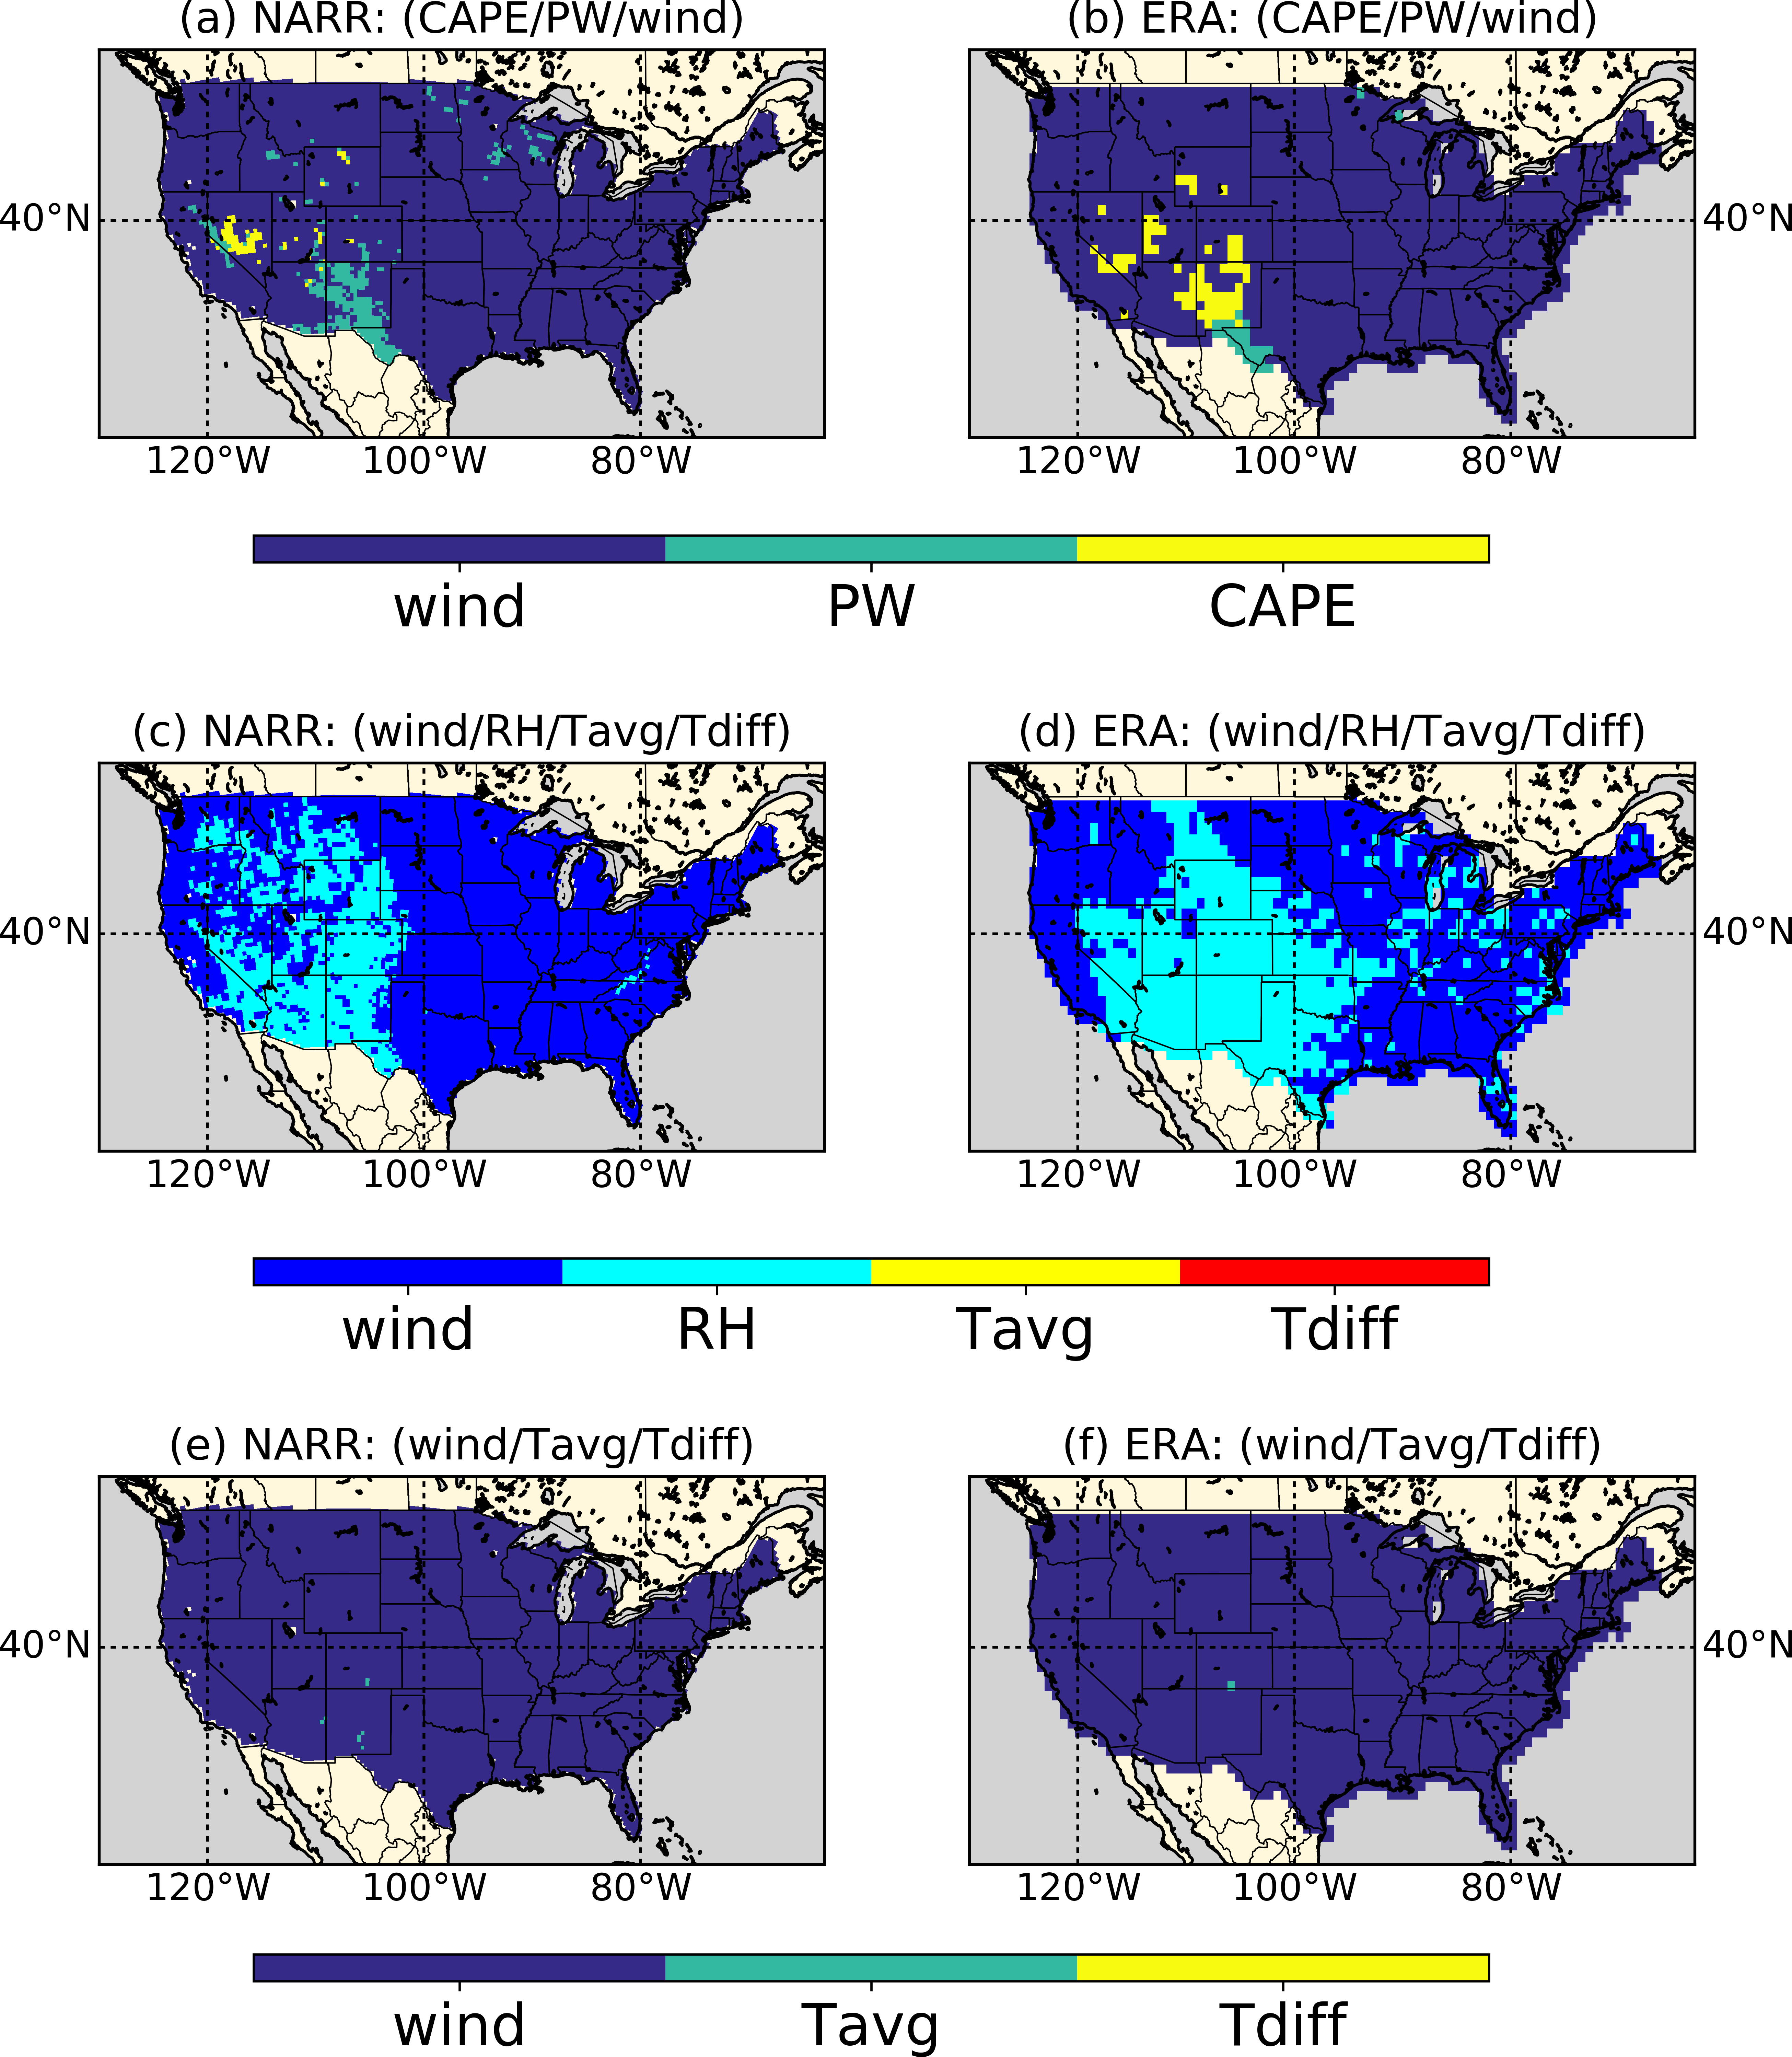
\includegraphics[width=\linewidth]{pics/ch4/fig5.png}
	\caption{Year-round dominant control over the extreme precipitation across CONUS. Panels (a) and (b) are analyses using $CAPE$/$PW$/$wind$, (c) and (d) are using $wind$/$RH$/$Tavg$/$Tdiff$, (e) and (f) are using $wind$/$Tavg$/$Tdiff$. Panels (a), (c), (e) are from NARR, (b), (d), (f) are from ERA-Interim.}
	\label{fig:4-5}
\end{figure}

Similarly, panels d-f of figure \ref{fig:4-5} shows the impact of distinct meteorological factors from NARR. They are $wind$ (c), $RH$ (d), average temperature (e) and temperature gradient (f). It is obvious that vertical wind and RH are the significant top two controls in general. Specifically, wind controls storms on the west coast and in the southeastern US, and $RH$ controls the mountainous region in the western US, as well as the Appalachian Mountains. The significant role of $RH$ is because $RH$ has a natural upper bound (of 100\%, or $\scriptsize{\sim}$105\% in supersaturation situations), and in the extreme precipitation duration, it often reaches this upper bound persistently. $PW$ is affected by two factors: $Tavg$ (i.e., the maximum moisture holding capacity) and $RH$ (how close the actual air moisture is to the maximum moisture holding capacity). Figure \ref{fig:4-4} indicates that $Tavg$ is not a key factor in driving $PW$ to an extreme condition in the precipitation (figure \ref{fig:4-5}b). $Tavg$ and $Tdiff$ have the most significant impact in the central-north US, around the Great Lakes. Also, $Tavg$ has a significant role in the southeast coastal regions and Florida.

\subsection{Year-round dominant controlling factor}

Based on figures \ref{fig:4-4} and \ref{fig:4-5}, we can now compare the strengths of relationship with various factors and pick a single factor that controls most of the 50 events as the dominant control of extreme 3-day precipitation at that grid. Figure \ref{fig:4-5} shows the distribution of such year-round dominant controls. Panels \ref{fig:4-5}a and \ref{fig:4-5}b paint the “competition” among general atmospheric conditions (atmospheric instability, moisture available and wind convergence). We can see that storms are mostly controlled by vertical wind (i.e., convergence) in general, though within the mountainous regions of the western US they would also be dominated by $CAPE$ or $PW$. Both NARR and ERA-Interim show similar patterns, except that ERA-Interim shows an expanded region that is dominated by $CAPE$. The $CAPE$/$PW$ dominant regions are distributed in the southwestern US, where the climate is dry and hot. Therefore, air tends to be dry and stable, requiring significant perturbation or abundant moisture influx before condensation can happen.

Panels c and d of figure \ref{fig:4-5} show the dominant meteorological factor in these precipitation events. Given that it is easier for $RH$ to reach its natural maximum (100\%) than $PW$, $RH$ exhibits dominant roles in the western US. In the meanwhile, the seasonal variation (i.e., the range between winter and summer values) of $RH$ is much smaller than other factors such as $Tavg$. Therefore, even for those extreme events occurring in winter, it would still be possible for $RH$ to reach its annual maximum. For these reasons, we performed another evaluation excluding $RH$, and the results are illustrated in panels e and f of figure \ref{fig:4-5}. It indicates that as $RH$ is taken out from the analysis, wind becomes the single domain-wide dominant factor. The domain-wide areas affected by $wind$ can also be partially explained by the weak seasonal cycle of wind, compared to $Tavg$ and $Tdiff$.

Though both NARR and ERA-Interim yield similar results, the major difference between the two is the contribution of wind. As seen in figure \ref{fig:4-5}d, over the mountainous western US, ERA-Interim gives fewer regions that are dominated by wind. This is likely due to the coarse horizontal resolution in ERA data, which makes it harder to elicit the finer scaled variation in wind speed as air flows over the mountainous regions. Another difference is the description of mesoscale convection systems (such as cyclones) in both datasets. In the ERA-Interim product, the 75-km horizontal grids fail to capture the spatial variability of cyclonic or tropical storm activity in the eastern US. Since such events contribute a considerable number of extreme precipitation events, the coarse resolution reanalysis indicates regions to be dominated by wind in the eastern US. Such impact from topography is also visible in figure \ref{fig:4-5}d, where the Pacific Northwest region (upper left region) in ERA-interim shows a continuous control under wind, while NARR successfully resolves the impact of the Cascade Range near the coast.

\subsection{Seasonality of dominant controls}

\begin{figure}[htbp]
	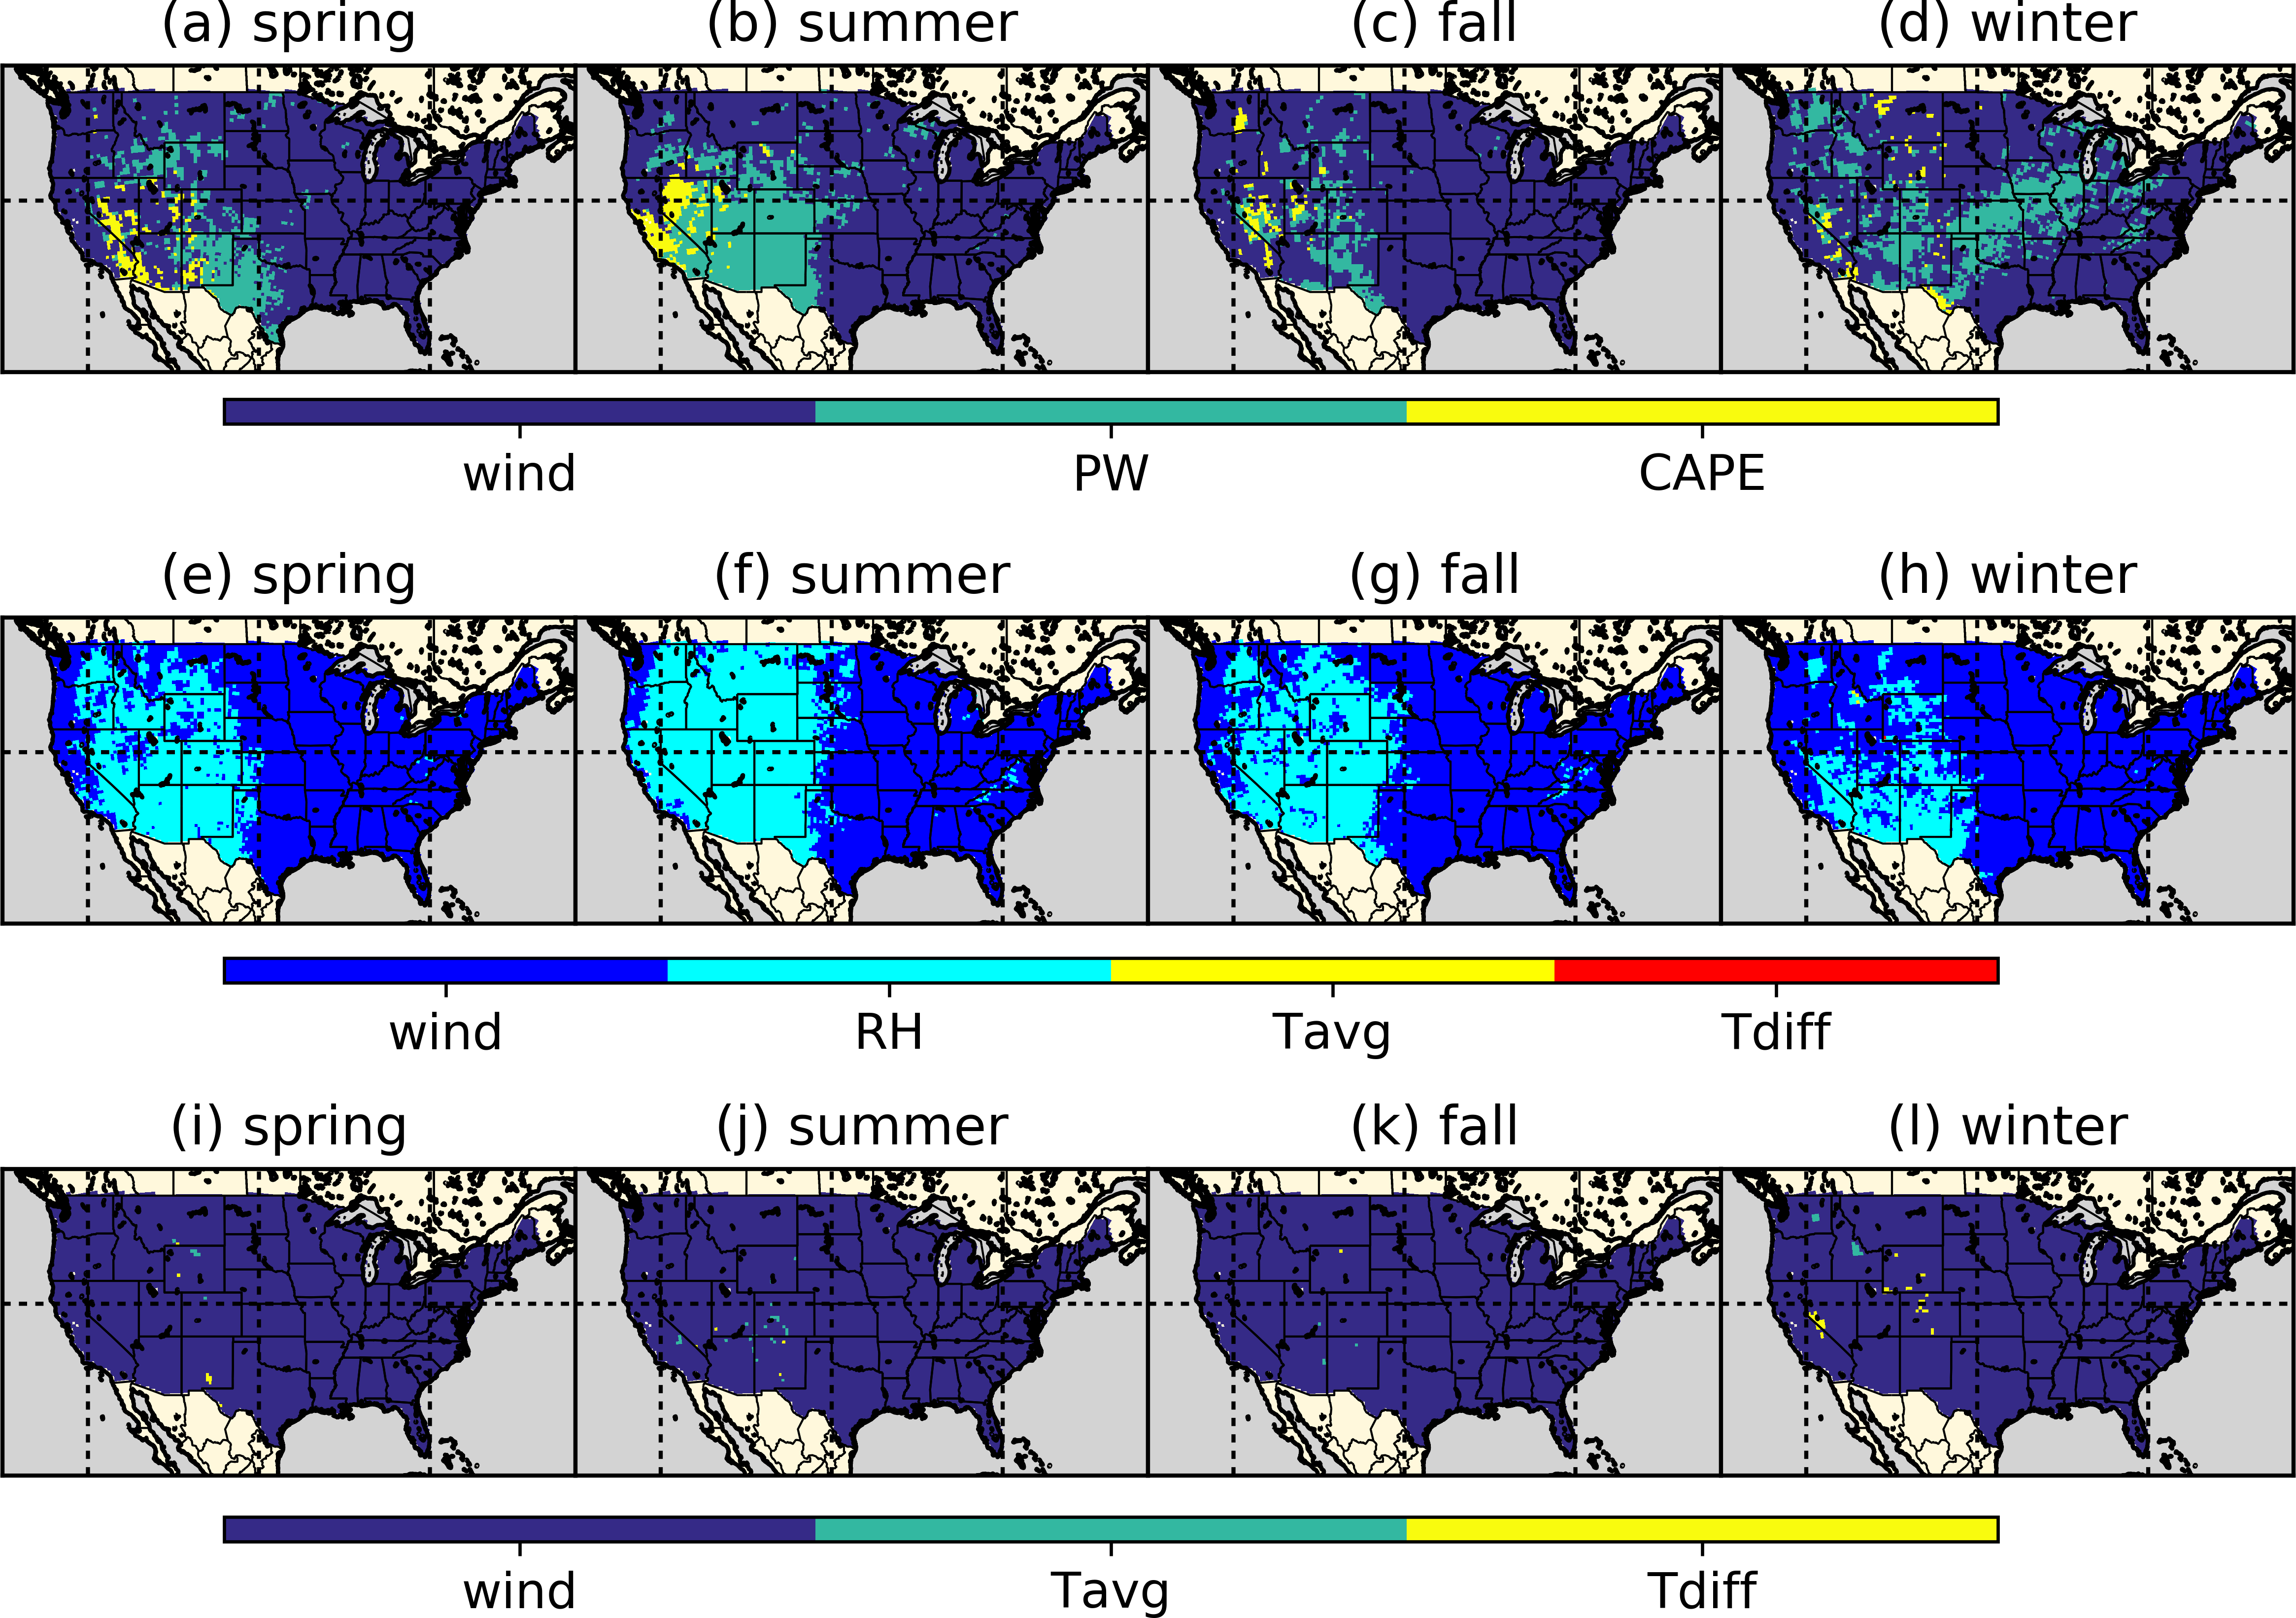
\includegraphics[width=\linewidth]{pics/ch4/fig6.png}
	\caption{Seasonal variations in the dominant controls, from NARR. The first row shows the seasonality among $wind$/$PW$/$CAPE$; the second row shows the seasonal variation among $wind$/$RH$/$Tavg$/$Tdiff$; the third row removes $RH$ from the analysis.}
	\label{fig:4-6}
\end{figure}

Figure \ref{fig:4-6} shows the seasonal variation in the dominant controls from NARR. For comparison, ERA-Interim results are shown in figure \ref{fig:4-S4}. Both reanalysis datasets show highly similar patterns, and they resemble the year-round patterns to a good extent. This simplifies the implementation of the finding in this study and indicates that the dominant factors found here are stable. In the $CAPE$/$PW$/$wind$ analysis, the southwestern US is more related to $PW$, since it is dry there in summer, and moisture controls the initialization of precipitation. Also, the northern US is controlled by $CAPE$ along with $wind$ in winter, as cold air is stable during winter. In terms of the $wind$/$RH$/$Tavg$/$Tdiff$ analysis, the patterns are stable across seasons. This is because $RH$ and $wind$, the two dominating factors, show less seasonal variability, and in all seasons it is easier for them to reach extreme.

The only big difference between the two reanalyses is during summer. NARR shows that the eastern US is controlled by $wind$, while ERA-Interim shows this region is now controlled by $RH$. Again, this is likely due to ERA-Interim failing to capture cyclones or tropical storms in the eastern US during summer when extreme precipitation is produced along with strong vertical winds. Therefore, the seasonality produced by NARR is more reliable.

\subsection{Inferring precipitation trends based on meteorological factors}

\begin{figure}[htbp]
	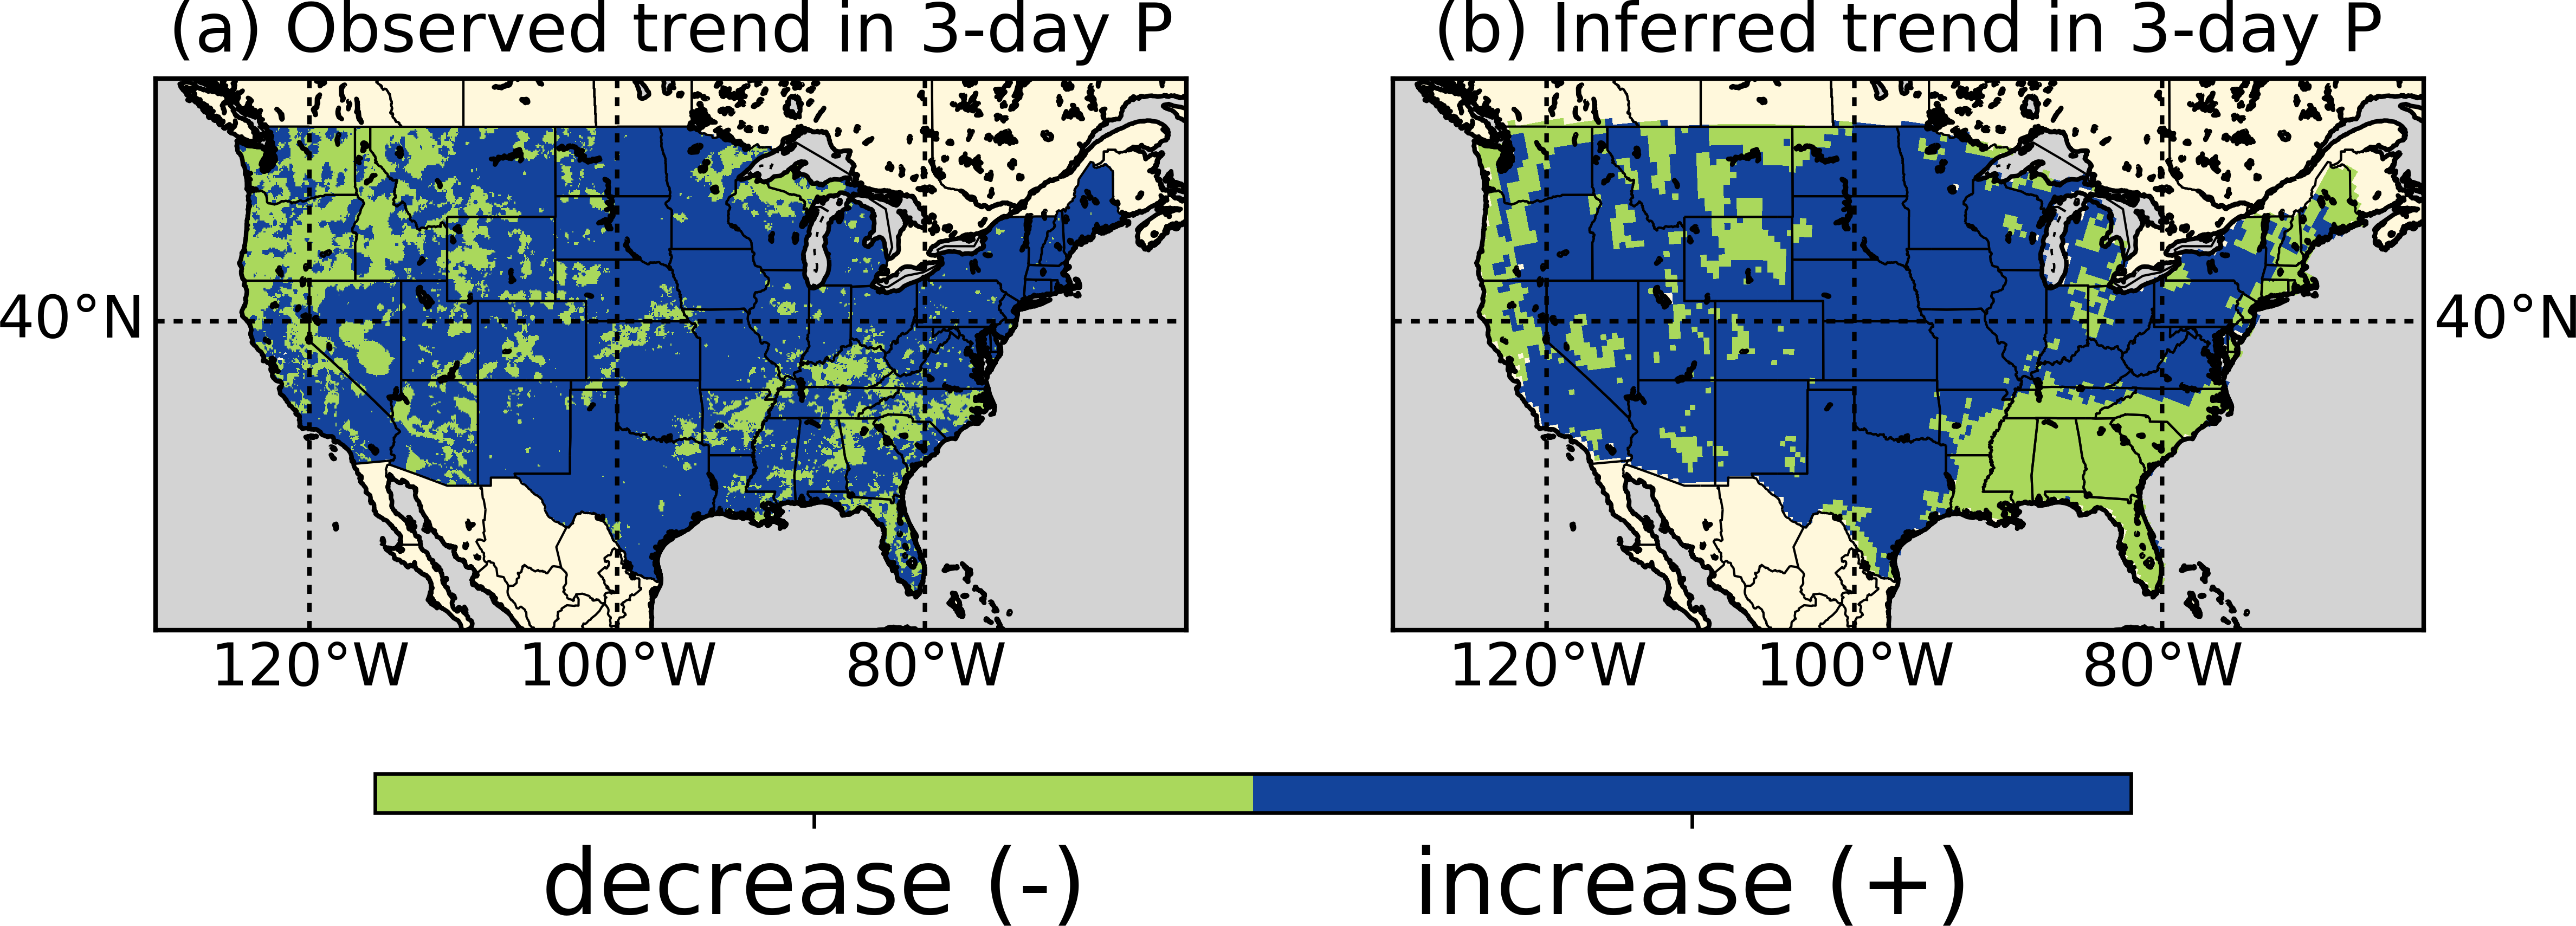
\includegraphics[width=\linewidth]{pics/ch4/fig7.png}
	\caption{Observed (a) and Inferred (b) binary trend of extreme 3-day precipitation. Panel (a) is the same as figure \ref{fig:4-3}a without actual trend value. Panel (b) is the inferred trend based on the dominant control map (figure \ref{fig:4-5}a), the trend in CAPE, PW and wind (figure \ref{fig:4-S2}). Details on the computation of this plot are in the method section.}
	\label{fig:4-7}
\end{figure}

The difficulty of precipitation simulation has been widely recognized in the climate modeling [\textit{IPCC}, 2001]. Given the year-round dominant control map in figure \ref{fig:4-5}a, it is possible to use the long-term trend of these factors in NARR to estimate the precipitation trends. In our analysis, if factor $X$ is the dominant control at a given grid, there is a positive relationship between extreme $X$ and extreme precipitation. Therefore, combining figure \ref{fig:4-5}a with the trends of these factors during 1979-2015 (figure \ref{fig:4-S2}), we can estimate the binary trends (i.e., increase or decrease) of extreme precipitation, the results are shown in figure \ref{fig:4-7}. As a validation, the trends derived from Livneh dataset are shown in figure \ref{fig:4-7}a. This is the same as figure \ref{fig:4-3}a, but with exact values removed. Figure \ref{fig:4-7}b shows the estimation based on the trends of meteorological factors. The large-scale spatial patterns show a good match: the vast regions in the middle and east US show increased precipitation; the northwest and southeastern US show decreased extreme precipitation. It is necessary to point out that figure \ref{fig:4-8}a is derived from 1/16 degree data, so it presents more variation at finer scales. Such good match suggests that it is possible to estimate the extreme precipitation trend from the long-term trends of related meteorological factors (that are easier to simulate reliably).

\section{Discussion}

For guidelines derived in this study as ready-to-use in engineering practice, they need to be robust and have an estimate of uncertainty. Here, we check the robustness of our results (both in the results themselves and how they compare to the previous studies). Also, as the guidelines are derived from relatively coarse resolution data (as compared with those high-resolution simulations suggested by climate modeling communities), the internal uncertainty in the simulated meteorological factors and thus the derived results are also investigated.

\subsection{Robustness check}

We checked the robustness of our results in three ways:

1) We checked the generated maps (figures \ref{fig:4-4}, \ref{fig:4-5} and \ref{fig:4-6}) using different thresholds. In the presented results, we used p1=95\% and p2=15\% (i.e., $CDF≥95\%$ and 15\% of 72-hour duration) as thresholds. We perturbed p1 between 90\% and 99\%, and p2 between 10\% and 20\% in the sensitivity experiments. The results (figure \ref{fig:4-S1}) are similar to figure \ref{fig:4-5}a.

2) We conducted the analysis using NARR and ERA-Interim data individually. The ERA-Interim results are shown in figure \ref{fig:4-5} and \ref{fig:4-S4}. Despite the difference in horizontal grid size (32 km and 75 km), the derived control maps share very similar spatial pattern.

3) We conducted another analysis, focusing on 1-day and 2-day extreme precipitation events. The derived maps of dominant atmospheric condition (figure \ref{fig:4-8}) resemble figure \ref{fig:4-5}. Thus the patterns we find here is robust for multi-day extreme precipitation events.

\begin{figure}[htbp]
	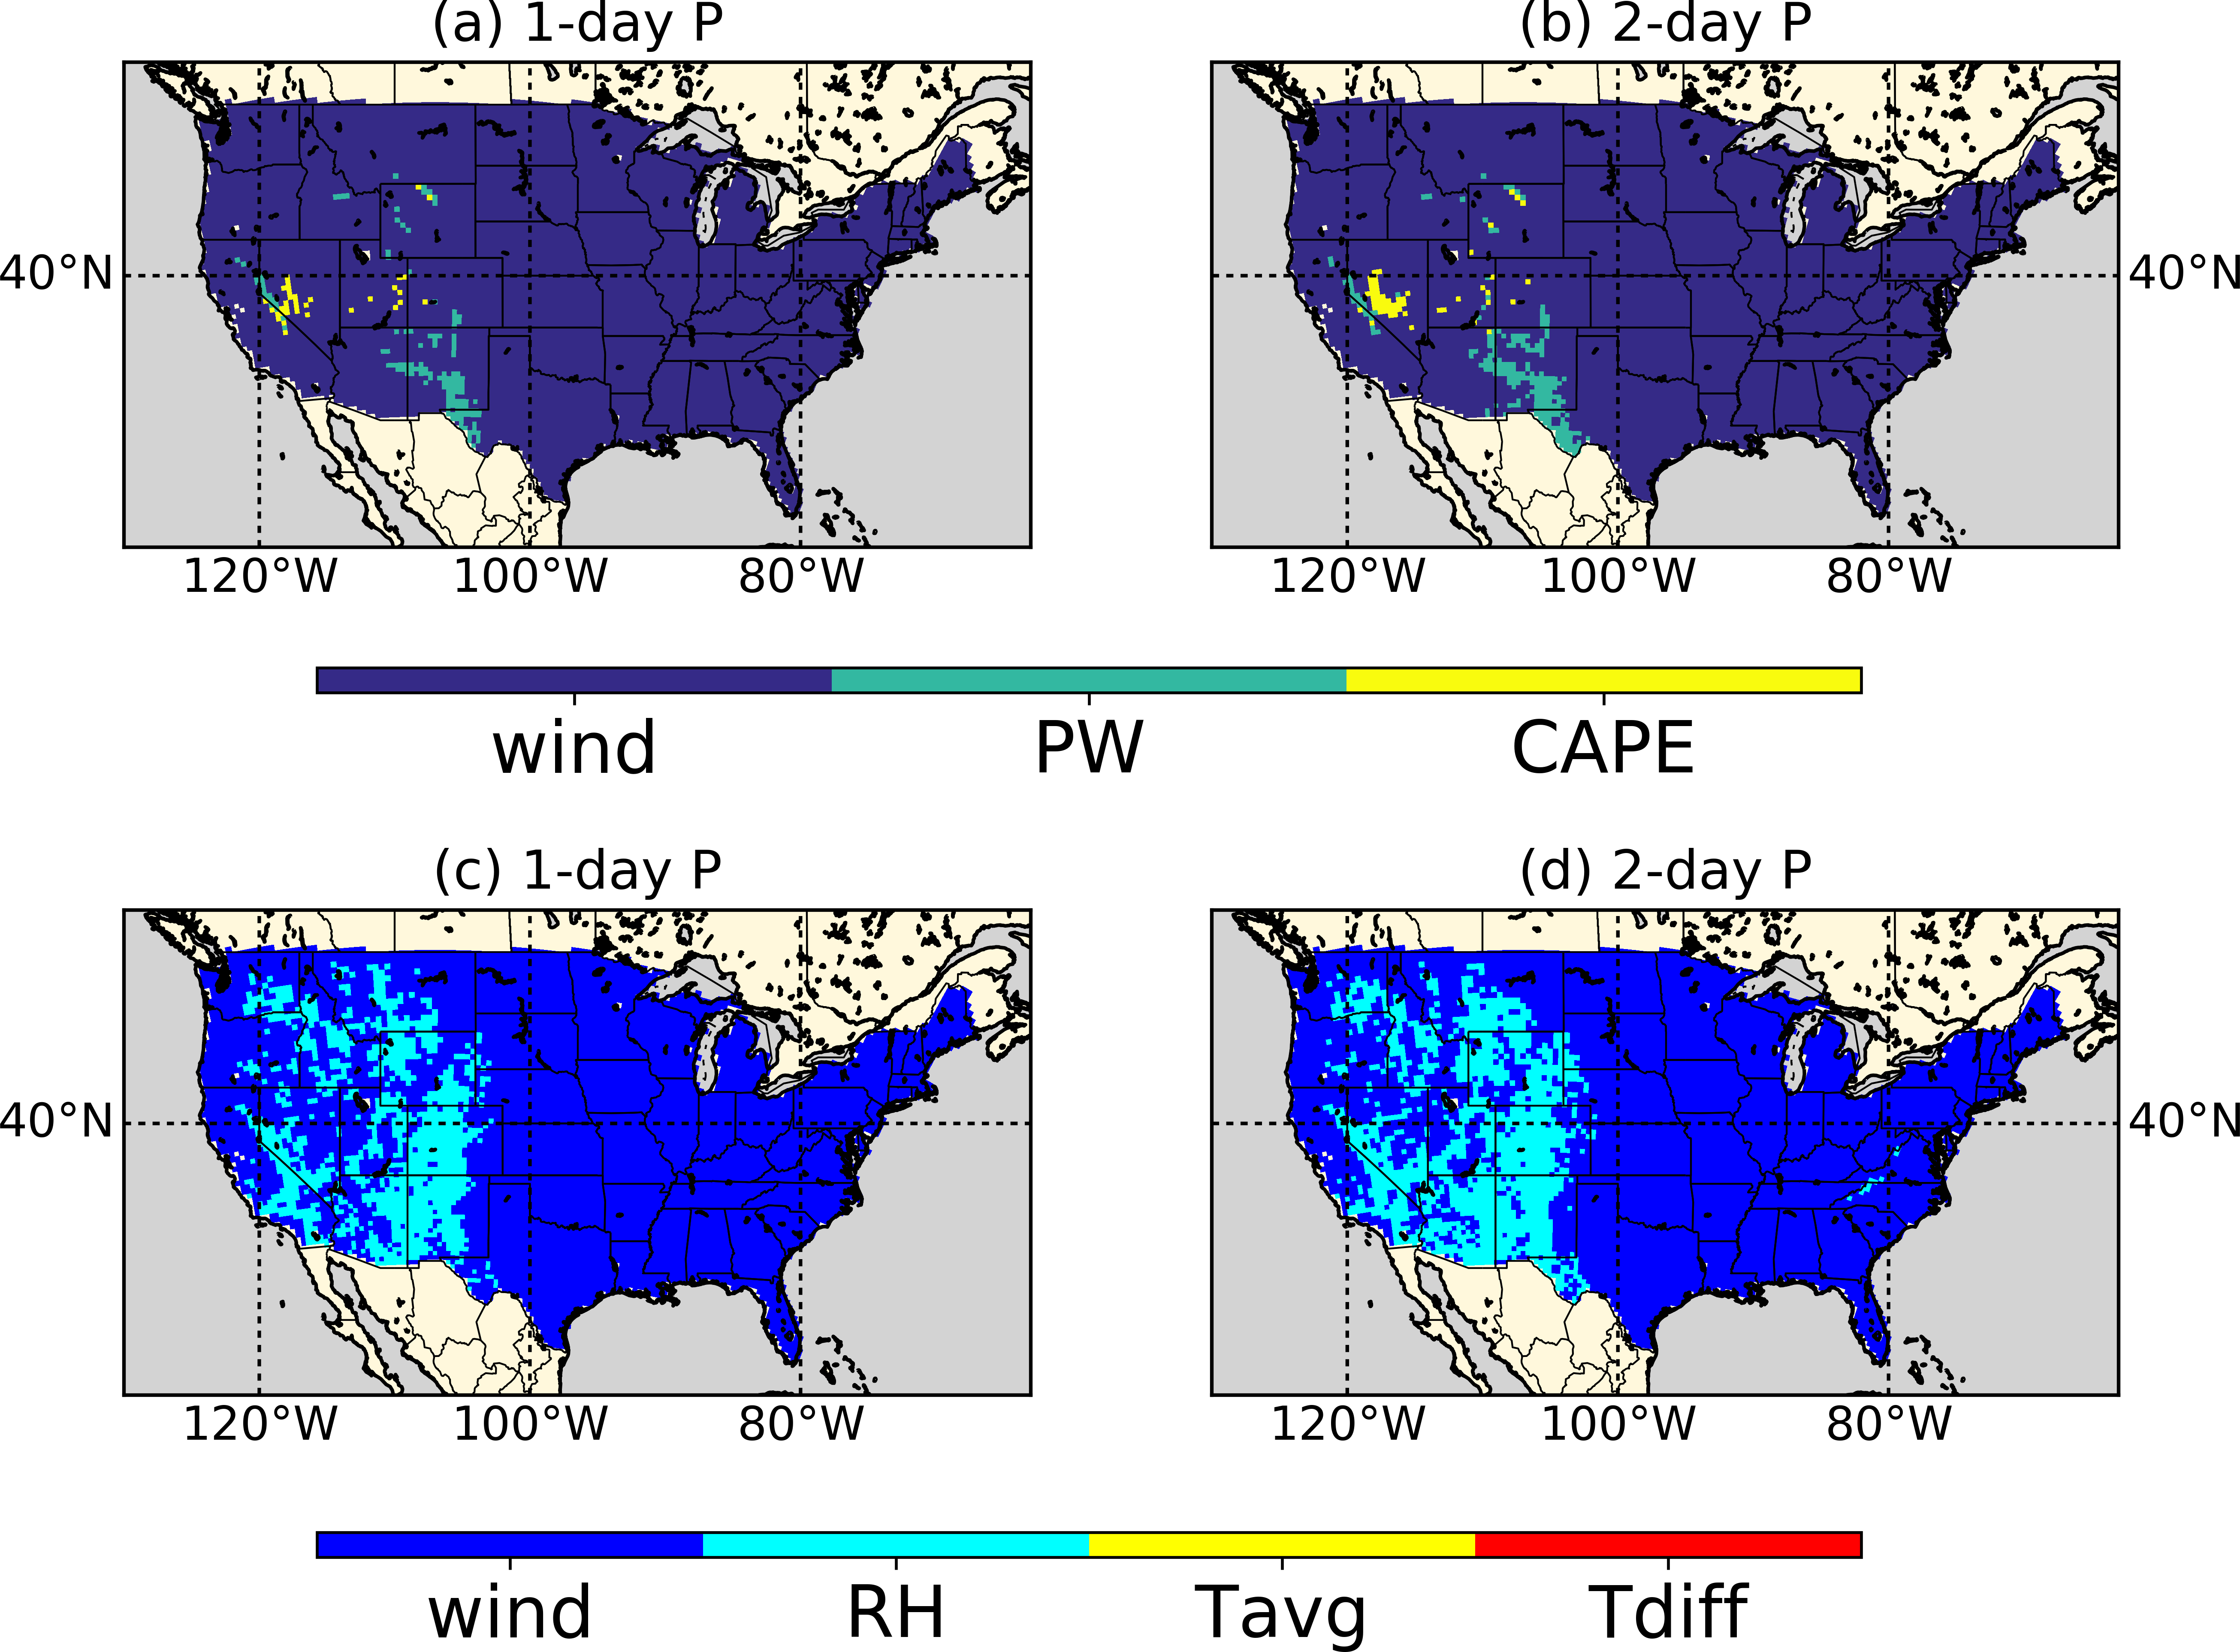
\includegraphics[width=\linewidth]{pics/ch4/fig8.png}
	\caption{Dominant atmospheric conditions in extreme 1-day and 2-day precipitation analysis. Panels (a) and (b) show the condition among $wind$/$PW$/$CAPE$, for 1-day and 2-day precipitation, respectively. Panels (c) and (d) are the analysis of $wind$/$RH$/$Tavg$/$Tdiff$.}
	\label{fig:4-8}
\end{figure}

\subsection{Spatial variations of physical controls}

Previous studies have checked the quantitative relationship between rainfall intensity and meteorological conditions [\textit{Mishra et al.}, 2012; \textit{Lepore et al.}, 2015; Loriaux et al., 2016]. Some of the studies regress the rainfall intensity P to moisture availability ($T_d$) and atmospheric instability ($CAPE$), and the results indicate that there is considerable variation in these regressions. For example, in the study of the US east of the Rocky Mountains (approximately east of 105ºW, see figure \ref{fig:4-S6}), the regression coefficient between $P$ and $T_d$ varies between 0.04-0.06 in 100-year return period extreme storms [\textit{Lepore et al.}, 2015].

Specifically, this coefficient is higher in the northeastern US (regions around the Great Lakes, “North” region in figure \ref{fig:4-S6}), and lower in the southeastern US (“South” in figure \ref{fig:4-S6}). This is consistent with our results that PW is related to more extreme storms in the northeastern US, while the relationship is weak in the southeastern US (figure \ref{fig:4-4}b). In terms of $CAPE$, the regression analysis indicates that P is most sensitive to $CAPE$ in the northeastern US (regions around the Great Lakes, “North” in figure \ref{fig:4-S6}), and the sensitivity decreases as it moves from north to south. Such gradient is also consistent with figure \ref{fig:4-4}a where storms in the north are more related to $CAPE$, but less in the southeast.

Compared to previous studies, we eliminated the biases introduced with different forms of regression. For example, some studies suggest that intensity of rainfall is positively related to $\sqrt{CAPE}$ [\textit{North and Erukhimova}, 2009], while others tried to regress rainfall intensity to $CAPE$ [\textit{Lepore et al.}, 2015]. In our approach, we only focus on the percentiles of $CAPE$ values, so the relationships derived (figure \ref{fig:4-4}) are free from assuming different forms of regression. Our results also suggest that the roles of these physical controls exhibit significant spatial heterogeneity, and they may need to be considered at a local scale to achieve even more reliable results.

\subsection{Uncertainty analysis}

While NARR is the highest resolution reanalysis available over the CONUS, the largest uncertainty in this analysis still originates from its relatively coarse resolution. It is known that such coarse resolution cannot fully resolve some of the mesoscale convective systems and tropical/extratropical cyclones. Also, the presentation of topography would lead to biases in the simulated moisture flow from cold season extreme precipitation in mountain regions [\textit{Prein et al.}, 2013]. To check the potential biases in our results, we performed the same analysis (but over only $PW$ and 700mb vertical velocity) over a 4-km WRF simulation across the CONUS during 2001-2012 [\textit{Liu et al.}, 2017]. As a reference, new maps based on 2001-2012 NARR data were also computed and shown in figure \ref{fig:4-9}. Panel \ref{fig:4-9}a is the percentage of top 50 storms that are related to extreme $PW$, \ref{fig:4-9}b is for vertical velocity. They are similar to panels \ref{fig:4-4}b and \ref{fig:4-4}c, but representative of the 2001-2012 period. Figures \ref{fig:4-9}c and \ref{fig:4-9}d are the results from WRF simulation. It shows that the $PW$ pattern in the 4-km grid simulation is similar to NARR result, so bias correction of $PW$ results is not necessary. For vertical wind, however, the WRF simulation indicates that over the western US, fewer storms are related to vertical velocity than that reflected in NARR results. Therefore, bias correction is required.

\begin{figure}[htbp]
	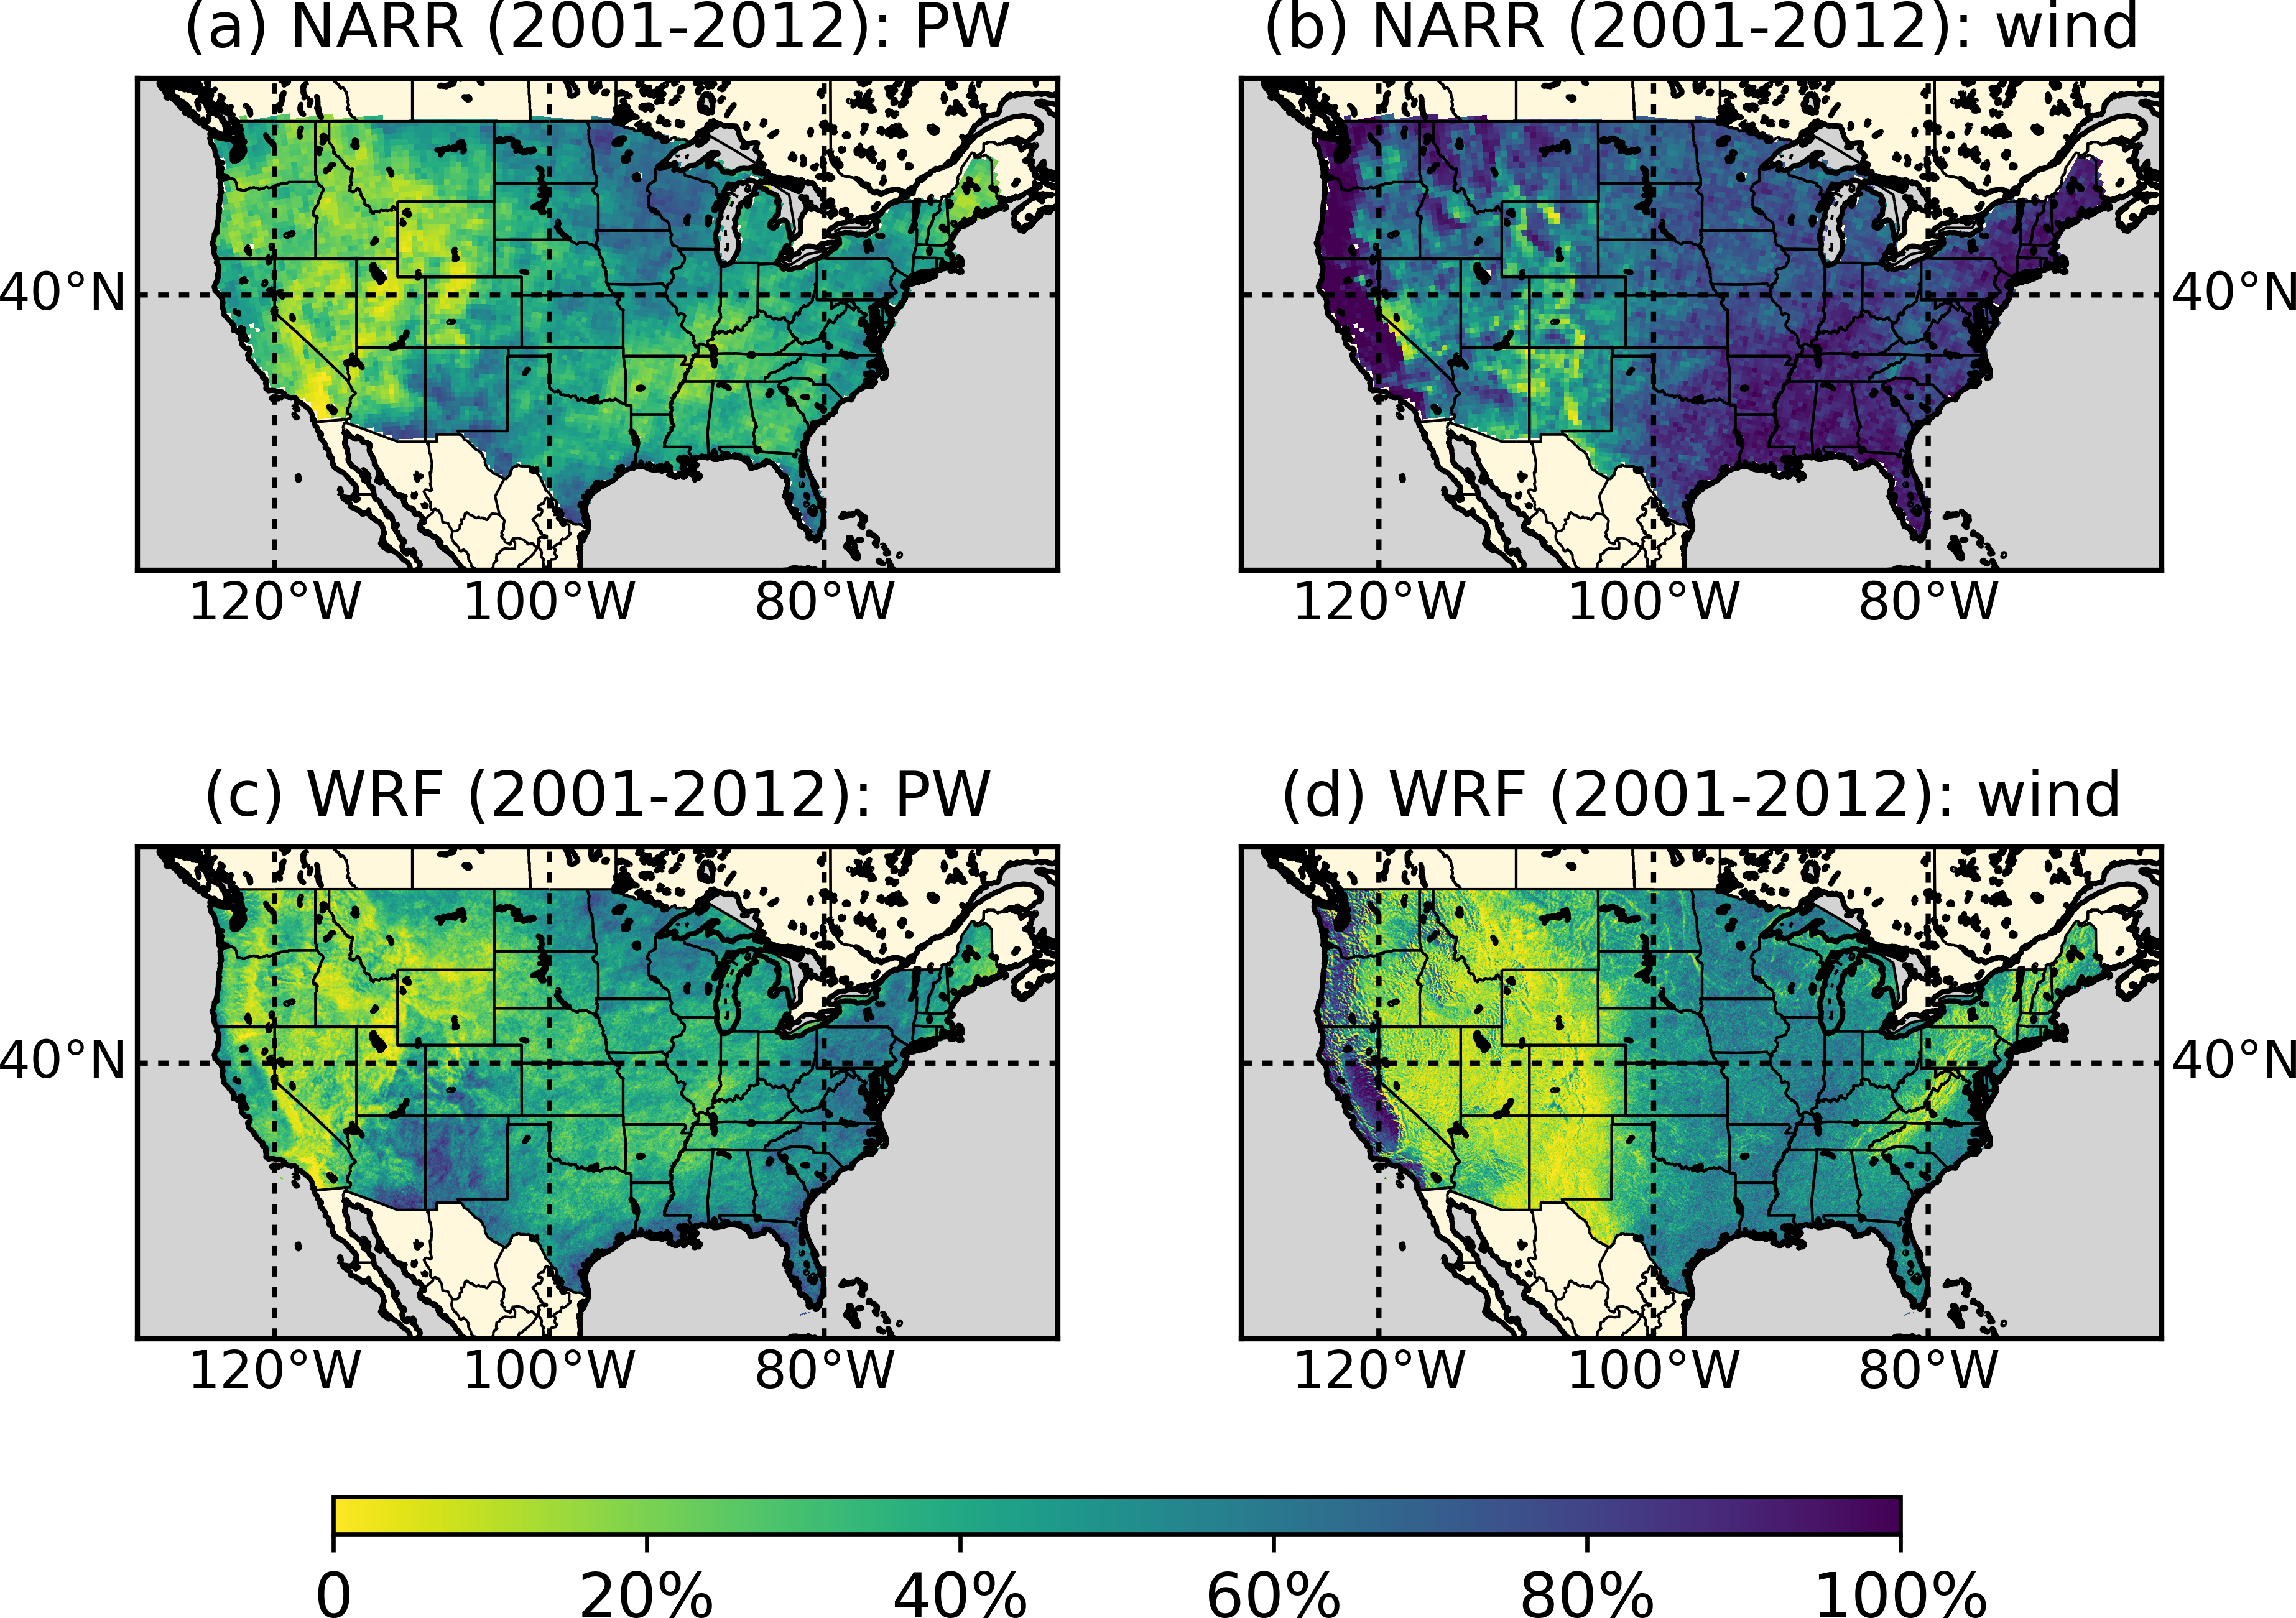
\includegraphics[width=\linewidth]{pics/ch4/fig9.png}
	\caption{Impact of reanalysis resolution on the analysis. Panel (a) is the analysis of $PW$, (b) is the analysis of $wind$, both are derived from 2001-2012 NARR data. Panel (c) and (d) are the analyses from a 4-km WRF simulation in the 2001-2012 duration (using ERA-Interim data as initial and boundary conditions).}
	\label{fig:4-9}
\end{figure}

Based on equation \ref{eq:4-3}, we can correct the wind percentage map in figure \ref{fig:4-4}c as:

\begin{equation}
pc{t_{NARR,bc}} = pc{t_{NARR,1979 - 2015}} + pc{t_{WRF,2001 - 2012}} - pc{t_{NARR,2001 - 2012}}
\label{eq:4-3}
\end{equation}


In equation \ref{eq:4-3}, $pc{t_{NARR,bc}}$ is the bias-corrected percentage, $pc{t_{NARR,1979 - 2015}}$ is the NARR percentage in figure \ref{fig:4-4}c, $pc{t_{WRF,2001 - 2012}}$ is the percentage derived from WRF (figure \ref{fig:4-9}d), $pc{t_{NARR,2001 - 2012}}$ is the percentage in 2001-2012 NARR data (figure \ref{fig:4-9}b). Using the bias-corrected wind percentage map, we can generate new dominant control map, as shown in figure \ref{fig:4-10}. Panel \ref{fig:4-10}a shows less dominant roles of vertical wind over the storms in the western US (excluding west coast). This makes more sense, as the Pacific Ocean provides moisture source for the extreme precipitation in this region. With the better presentation of topographic impact in the model, moisture tends to be lifted and condensed as they travel above the Rocky Mountains. Therefore, it is critical to have enough moisture retained in the airflow for the precipitation to happen in the western US. The big patterns between panel \ref{fig:4-10}b and \ref{fig:4-5}c are similar, though the better description of the Appalachian Mountains now results in less wind control in this region.

\begin{figure}[htbp]
	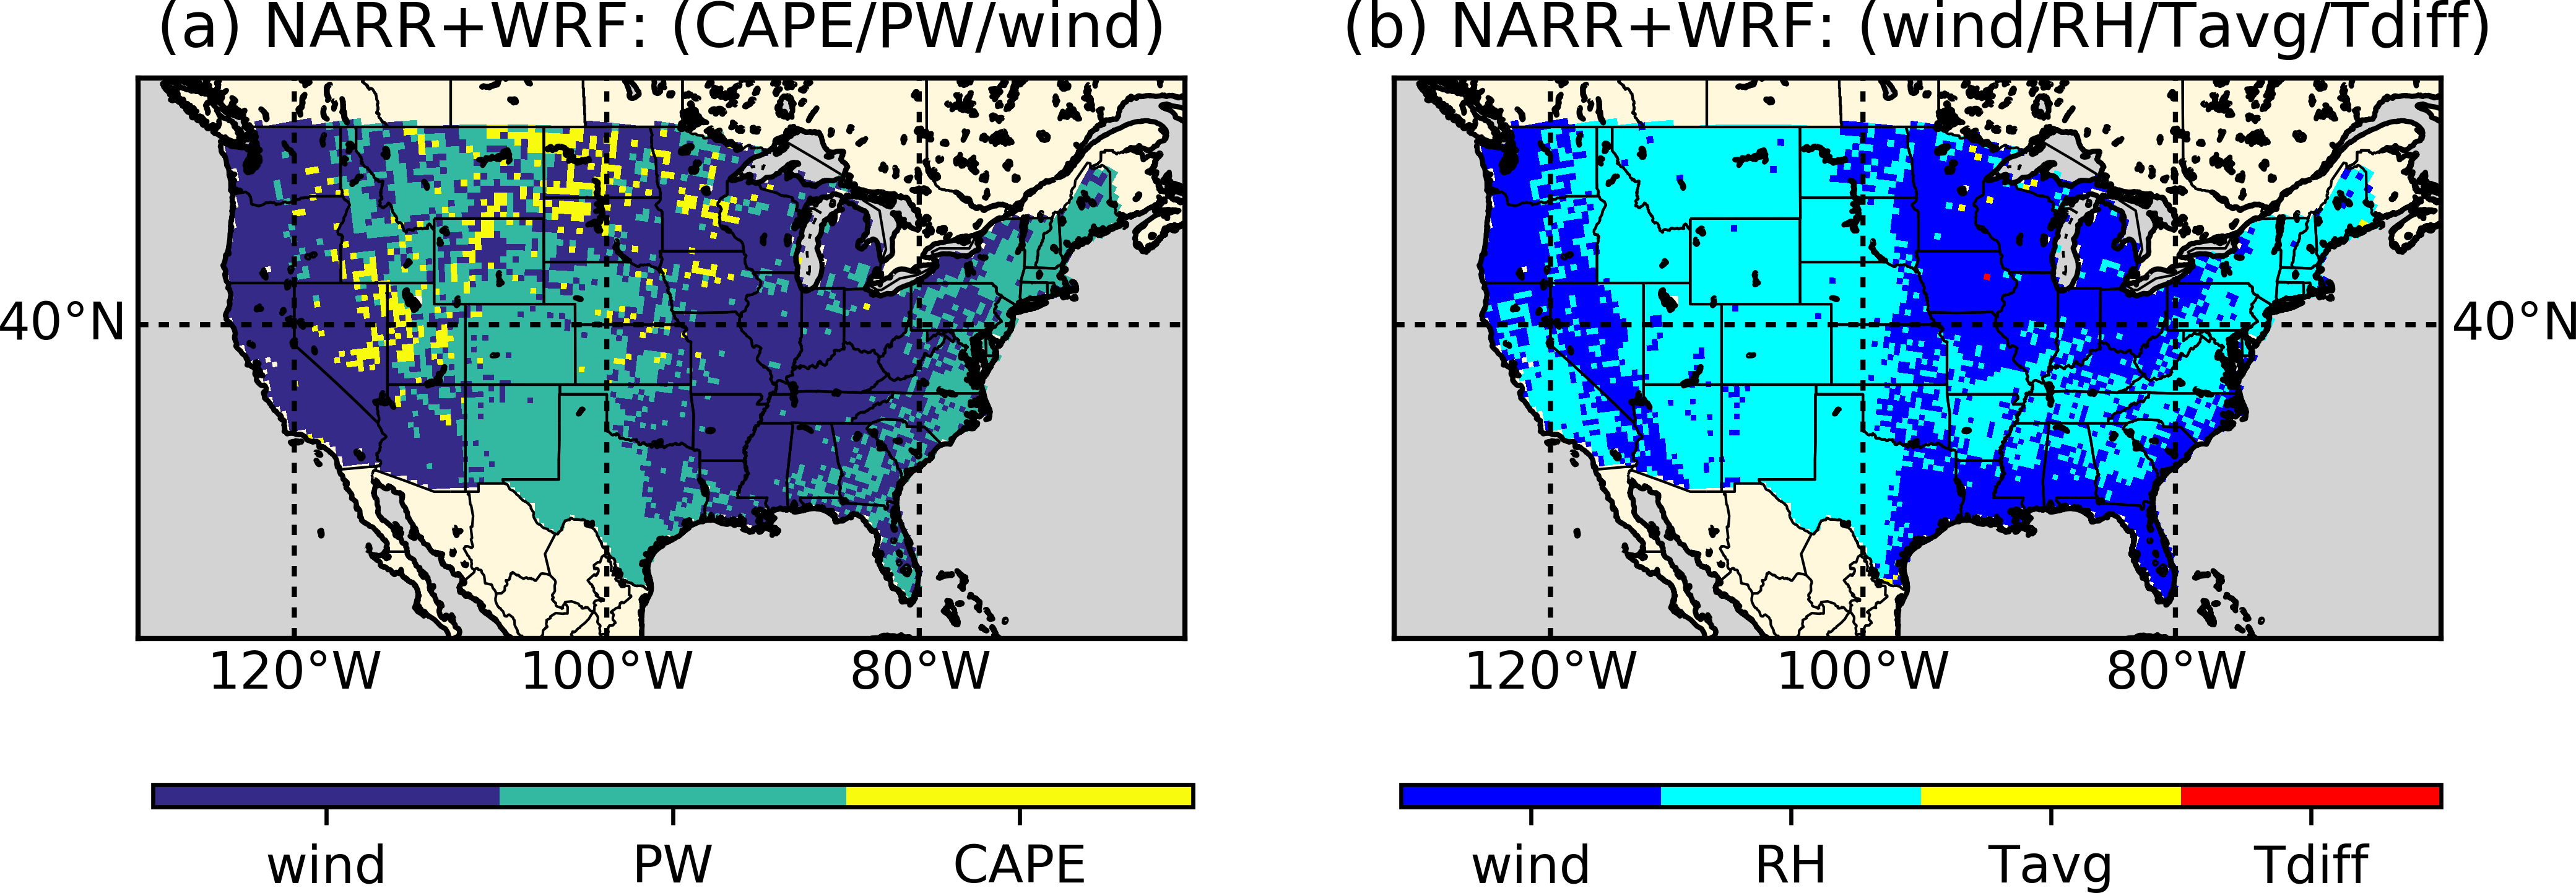
\includegraphics[width=\linewidth]{pics/ch4/fig10.png}
	\caption{Dominant meteorological conditions derived from NARR and 4-km WRF simulation. $wind$ results (i.e., figure \ref{fig:4-4}c) are corrected using 4-km WRF simulation (2001-2012), and the other percentage results are as obtained from 1979-2015 NARR analysis (figure \ref{fig:4-4}). Details on the correction of wind results are described in the discussion section.}
	\label{fig:4-10}
\end{figure}

\subsection{Model-based PMP estimation}

As mentioned earlier, the main motivation of our study is the recent advances in PMP estimation using numerical atmospheric models. Despite various efforts to investigate how to use models to maximize the extreme historical rainstorms to PMP level [\textit{Tan}, 2010; \textit{Ohara et al.}, 2011; \textit{Ishida et al.}, 2015], there has been no general agreement reached so far within the community. Various maximization approaches have been applied to various storms, but the extent they maximize the storms differ a lot. Considering the spatial variation of physical controls shown in figure \ref{fig:4-5} and \ref{fig:4-7}, this is likely due to the different dominant controls on the storms at different locations. For example, \textit{Ohara et al.} [2011] tested several methods over the 1997 January storm in central California (American River Watershed) and found that perturbation of horizontal wind convergence produced much larger “PMP storm” than increasing relative humidity to 100\%. This result can be explained by figure \ref{fig:4-5}a where central and south California is mainly controlled by the vertical wind velocity. At the same time, \textit{Ohara et al.} [2017] found that increasing $RH$ to 100\% sometimes leads to decreased precipitation. This can now also be explained by the dominant role of vertical $wind$ (rather than $PW$) at this location. At $wind$-control locations, disturbance of wind speed would greatly change the rainfall magnitude, while at $PW$-control locations rainfall magnitude will change more under air moisture change. On the other hand, $RH$ is the only considered driver that gets maximized in the model. This makes sense for the western US (excluding the west coast area) if we look at figures \ref{fig:4-6}c and \ref{fig:4-6}d where $RH$ dominates the western US. However, $RH$ has a physical upper bound (100\%), and it is often already 100\% in the storm duration, so maximizing it cannot fully release the precipitation potential. This may also explain why the model-based PMP estimation using $RH$ maximization tends to be lower than the value from NOAA’s operational guideline Hydrometeorology Reports (HMR) [\textit{Tan}, 2010; \textit{Ohara et al.}, 2011]. In HMR, we maximize the precipitation using $PW$, while $RH$ is only a factor in $PW$. Therefore, it is important to determine the key control of the rainstorms over the study region and release this constraint in the model accordingly.

Based on our analysis, we suggest that $RH$ should be the first value to be maximized in model-based 3-day PMP estimation. Since $RH$ has a natural limit of 100\%, setting $RH$ to 100\% does not necessarily amplify the storm to its upper bound. In this case, considering the second factor would be useful: $wind$ field is an important factor to consider in the model. By setting the $wind$ fields to its climatological maxima, precipitation would be amplified to a reasonably higher amount. Such numbers should make a safer and more physics-based PMP estimate. For more detailed PMP design, it may be worthwhile to check the dominant controls at seasonal (or even monthly) scale and finer-resolution regional climate simulation when available, and then run the models accordingly.

In this study, we have provided data-driven rationale and guidance to engineers on what physical triggers would make the most justification in configuring a numerical model for estimating 3-day PMP. Based on similarities between figure \ref{fig:4-5} and figure \ref{fig:4-8}, such guidance is also valid for 1-day and 2-day PMP estimation. For PMP estimation of other different durations, the frequency-based analysis framework we introduced here can be used to identify the key controlling factors.

\section{Conclusions}

We used the NARR and ERA-Interim reanalysis to investigate the roles of general atmospheric conditions (instability, moisture availability, wind convergence) and atmospheric drivers (vertical wind, relative humidity, air temperature) in extreme rainstorm events. These relationships bring the guidelines towards a physics-based PMP estimation framework. Our conclusions are:

1.	Extreme 3-day precipitation shows different trends across the CONUS. Central US shows a significant increase during 1948-2010. The extreme precipitation in western US and part of the southeastern US has a decreasing trend over time, although the southeastern US decrease appears statistically non-significant. This can be explained by strong relationship between extreme precipitation and vertical wind velocity across the US;

2.	Both reanalysis datasets show that extreme storms across much of CONUS are closely related to vertical wind velocity. Storms in the southwestern US is more related to moisture availability and atmospheric instability;

3.	From the perspective of atmospheric driving factors, relative humidity and vertical wind have a domain-wide impact over the extreme precipitation. The roles of these factors do not exhibit strong seasonality;

4.	The engineering and water infrastructure community can use numerical models to physically estimate probable maximum precipitation after properly considering the existing major controls on the extreme storms (i.e., $RH$ and $wind$). This will help to provide more solid model-based PMP estimates.

For a physics-based PMP estimation framework across the CONUS, we find two flaws in the RH maximization methods that has been proposed by many in numerical modeling studies in the past: 1) RH may not be the major factor that mostly relate to the extreme precipitation, especially in the eastern US where storm magnitudes are more related to the vertical wind velocity; 2) due to its natural upper bound ($\scriptsize{\sim}$100\%), it cannot maximize the extreme precipitation to its maximum extent. Here we suggest that besides the RH maximization, the vertical wind fields maximization is also required for a reliable PMP estimation. By generating the map on the spatial distribution of dominant controls (figure \ref{fig:4-5}), we also provide guidelines for the engineering community on which factor should be prioritized in different regions across the CONUS.

Our study opens the way for physics-based 3-day PMP estimation in the CONUS. At the same time, the frequency-based analysis framework of the study can also be applied to storm analysis at various durations and in other regions where high-resolution climate reconstruction (such as the most recent ERA-5 reanalysis product) is available. Our study provides a solid and evidence-based guideline to engineers for modernizing PMP estimation using numerical models and state of the art in atmospheric science.

Up to this point, the physics-based PMP estimation approach is established. However, a problem still exists: For the site that traditional approach estimates PMP as 1000mm, if the physics-based approach estimates the current PMP as 800mm while future PMMP as 900mm, is the infrastructure at this site safe in the future? In other words, how to understand the difference between traditional and physics-based PMP estimations? We will explore this in the next chapter.